\documentclass[12pt]{book}
\usepackage[T1]{fontenc}
\usepackage{times}
\usepackage{listings}
\usepackage{graphicx}
\usepackage{xcolor}
\usepackage{url}
\usepackage{booktabs}
\usepackage{array}
\usepackage{longtable}
\usepackage{float}
\usepackage{url}
\usepackage{etoolbox}  % for showidx
\usepackage{fullpage}
\usepackage{soul}
\usepackage[utf8]{inputenc}
\usepackage{amsmath}

\usepackage{tikz}
\usetikzlibrary{shapes,arrows,positioning}
\usetikzlibrary{arrows.meta}
\usepackage{adjustbox}

\usepackage{hyperref}  % should be last
\definecolor{linkblue}{rgb}{0.05,0.25,0.65}
\hypersetup{
  pdfborder={0 0 0},
  colorlinks=true,
  linkcolor=linkblue,
  citecolor=linkblue,
  urlcolor=linkblue
}

\definecolor{codegreen}{rgb}{0,0.6,0}
\definecolor{codegray}{rgb}{0.5,0.5,0.5}
\definecolor{codepurple}{rgb}{0.58,0,0.82}

\lstdefinestyle{mystyle}{
    commentstyle=\color{codegreen},
    keywordstyle=\bfseries\color{magenta},
    stringstyle=\color{codepurple},
    basicstyle=\ttfamily\footnotesize,
    showstringspaces=false,
    xleftmargin=0.5cm
}
\lstset{style=mystyle}
\lstset{captionpos=b}

% Syntax highlighting for OctaC source: keywords (magenta, bold),
% line comments (green), no background shading.
\lstset{
    morekeywords={function, return, if, else, for, in, until, do, and, or,
                  not, is, true, false, i32, i64, f32, f64, bool, matrix,
                  vector, elseif, caseof, case, i16, default, break,
                  continue, f16, string},
    morecomment=[l]{//},
    morestring=[b]"
}

\usepackage{xstring}

% A bare state or token name in monospace, allowed to break after
% underscores: \stok{START}, \stok{STAR_SLASH_MOD}.
%
% A token in <class, value> or <class,> form, built from the class name and
% an optional value: \tok{START} -> <START,>, \tok{SCALAR, i32} ->
% <SCALAR, i32>. The class name is broken at underscores as in \stok.
\makeatletter
\def\tok@split#1_#2\@nil{#1\if\relax\detokenize{#2}\relax\else\_\allowbreak\tok@split#2\@nil\fi}
\newcommand{\stok}[1]{\texttt{\tok@split#1_\@nil}}
\def\tok@pair#1, #2\tok@stop{\texttt{<\stok{#1},}\,\texttt{#2>}}%
\newcommand{\tok}[1]{%
  \IfSubStr{#1}{,}%
    {\tok@pair#1\tok@stop}%
    {\texttt{<\stok{#1},>}}%
}
\makeatother

% A nonterminal of the grammar, set in italics: \nt{Expr}.
\newcommand{\nt}[1]{\textit{#1}}

% Style for pseudocode listings: the same keyword/string highlighting as
% real code, but for control-flow words instead of OctaC's keywords.
\lstdefinestyle{pseudocode}{
    keywords={function, switch, case, default, return, new, throw,
              catch, try, if, else, while, for, break, continue},
    keywordstyle=\bfseries\color{magenta},
    stringstyle=\color{codepurple},
    commentstyle=\color{codegreen}
}

% One space after periods
\frenchspacing

% Do not stretch vertical space to fill pages, so unbreakable blocks
% (tables, listings) never leave large gaps around them.
\raggedbottom

\hypersetup{pdfauthor={Syed Taha, Muhammad Usman},
            pdftitle={OctaC: A Language Specification},}

\lstset{basicstyle=\small\ttfamily}
\lstset{escapeinside={(*@}{@*)}}
\lstset{xleftmargin=5.0ex}

\newcommand{\github}{https://github.com/mit-pdos/xv6-riscv/blob/riscv/}

\newcommand{\fileref}[1]{\small{\textcolor{red}{(#1)}}}
\newcommand{\lineref}[2]{\small{\textcolor{red}{(#1:#2)}}}
\newcommand{\linerefs}[3]{\small{\textcolor{red}{(#1:#2-#3)}}}

\newcommand{\showfileref}[2]{\href{\github/#1}{\small{(\textcolor{blue}{#2})}}}
\newcommand{\showlineref}[3]{\href{\github/#1\#L#2}{\small{(\textcolor{blue}{#3})}}}
\newcommand{\showlinerefs}[5]{\href{\github/#1\#L#2-L#3}{\small\textcolor{blue}{(#4-#5)}}}

%% editing markup
\newcommand{\insertnote}[3]{\noindent\textcolor{#1}{\textbf{#2:} #3}}
\newcommand{\note}[1]{\insertnote{blue}{NOTE}{#1}}

% ------------------------------------------------------------
% Inline code styling
% ------------------------------------------------------------
\usepackage[most]{tcolorbox}

\tcbset{
    myinlinecode/.style={
        enhanced,
        boxsep=0.3mm,
        left=0.5mm,
        right=0.5mm,
        top=0.5mm,
        bottom=0.5mm,
        colback=gray!20, % background color
        colframe=gray!20, % optional border color
        arc=1mm,          % rounded corners
        boxrule=0pt,    % border thickness
        box align=base,   % aligns nicely with text
        before skip=0pt,
        after skip=0pt,
        fontupper=\ttfamily % monospace font
    }
}

% Command for easier usage
\newtcbox{\code}{myinlinecode, tcbox raise=0pt, box align=base, on line}

\title{\textbf{OctaC: A Language Specification}\\[0.3em]
\large Designing a Hybrid Language for Numerical and Matrix Computation}
\author{Syed Taha \and Muhammad Usman}

\begin{document}

\maketitle

{\hypersetup{linkcolor=black}\tableofcontents}

\input{acks}
\addcontentsline{toc}{chapter}{Foreword and acknowledgments}

\input{preface}
\addcontentsline{toc}{chapter}{Preface}

%  Part 1: Language Design
\part{Language Design}
\input{p1-chp01-introduction}
% p1-chp02-lexer.tex

\chapter{Lexical Analysis and the Lexer}
\label{chp:lexer}

The lexical analyzer, or lexer, is the first phase of the compiler. It reads
the source program as a stream of characters and groups them into tokens,
the units that the parser works with \cite{aho2006compilers}. This chapter
defines the full token specification of OctaC, the deterministic finite
automata that recognize those tokens
\cite{aho2006compilers,hopcroft2006automata}, and the algorithm the lexer
uses to drive them. The source code of the lexer is available at:
\url{https://github.com/Octa-C/compiler/tree/main/lexer}

\section{Token Specification}

This section lists the complete token set for the lexical analyzer, in
Table~\ref{tab:token-set}. Every token belongs to a category, and some
belong to a subcategory within it: the loop keywords \code{for}, \code{do},
\code{until}, and \code{continue}, for example, belong to the Keyword
category and the Loops subcategory. The Token column gives the token as it
is written in the source, or a descriptive name where one token covers
several lexemes. The Values column is filled only for those tokens that
match more than one lexeme, or a pattern, such as the scalar datatypes or
the integer literals, and lists the lexemes or the regular expression they
match. The last column gives the generated name of the token, a short
capitalized name such as \code{FOR} or \code{ASSIGNMENT}, which is the name
used to identify the token from here on.

The logical and equality operators are written as English words, so they are
listed among the keywords rather than the operators. The two compiler tokens,
EOF and Error, do not correspond to any source text and are produced by the
lexer itself.

\begin{table}[tbp]
\centering
\fontsize{6.2}{7.2}\selectfont
\renewcommand{\arraystretch}{1.1}
\setlength{\tabcolsep}{2pt}
\begin{tabular}{@{}ll@{\hspace{6pt}}ll@{\hspace{6pt}}l@{}}
\toprule
\textbf{Category} & \textbf{Subcategory} & \textbf{Token} & \textbf{Values} & \textbf{Generated token} \\
\midrule
Keyword & Loops & \texttt{for} &  & \stok{FOR} \\
Keyword & Loops & \texttt{do} &  & \stok{DO} \\
Keyword & Loops & \texttt{until} &  & \stok{UNTIL} \\
Keyword & Loops & \texttt{continue} &  & \stok{CONTINUE} \\
Keyword & Function & \texttt{function} &  & \stok{FUNCTION} \\
Keyword & Function & \texttt{return} &  & \stok{RETURN} \\
Keyword & Conditional & \texttt{if} &  & \stok{IF} \\
Keyword & Conditional & \texttt{else} &  & \stok{ELSE} \\
Keyword & Conditional & \texttt{elseif} &  & \stok{ELSEIF} \\
Keyword & Conditional & \texttt{caseof} &  & \stok{CASEOF} \\
Keyword & Conditional & \texttt{case} &  & \stok{CASE} \\
Keyword & Conditional & \texttt{default} &  & \stok{DEFAULT} \\
Keyword & Word-based Logic/Rel Ops & \texttt{and} &  & \stok{AND} \\
Keyword & Word-based Logic/Rel Ops & \texttt{or} &  & \stok{OR} \\
Keyword & Word-based Logic/Rel Ops & \texttt{not} &  & \stok{NOT} \\
Keyword & Word-based Logic/Rel Ops & \texttt{is} &  & \stok{IS} \\
Keyword & Word-based Logic/Rel Ops & \texttt{in} &  & \stok{IN} \\
Keyword & Misc & \texttt{break} &  & \stok{BREAK} \\
\midrule
Datatype &  & Scalar & \texttt{i64}, \texttt{i32}, \texttt{i16}, \texttt{f64}, \texttt{f32}, \texttt{f16}, \texttt{bool} & \stok{SCALAR} \\
Datatype &  & \texttt{vector} &  & \stok{VECTOR} \\
Datatype &  & \texttt{matrix} &  & \stok{MATRIX} \\
Datatype &  & \texttt{string} &  & \stok{STRING} \\
\midrule
Punctuation &  & \texttt{\{} &  & \stok{LBRACE} \\
Punctuation &  & \texttt{\}} &  & \stok{RBRACE} \\
Punctuation &  & \texttt{(} &  & \stok{LPAREN} \\
Punctuation &  & \texttt{)} &  & \stok{RPAREN} \\
Punctuation &  & \texttt{[} &  & \stok{LBRACKET} \\
Punctuation &  & \texttt{]} &  & \stok{RBRACKET} \\
Punctuation &  & \texttt{;} &  & \stok{SEMICOLON} \\
Punctuation &  & \texttt{->} &  & \stok{ARROW} \\
Punctuation &  & \texttt{,} &  & \stok{COMMA} \\
Punctuation &  & \texttt{...} &  & \stok{ELLIPSIS} \\
Punctuation &  & \texttt{:} &  & \stok{COLON} \\
\midrule
Operators & Standard & \texttt{+-} & \texttt{+}, \texttt{-} & \stok{PLUSMINUS} \\
Operators & Standard & \texttt{* / \%} & \texttt{*}, \texttt{/}, \texttt{\%} & \stok{STAR_SLASH_MOD} \\
Operators & Matrix & \texttt{'} &  & \stok{TRANSPOSE} \\
Operators & Matrix & \texttt{.*} &  & \stok{DOT_STAR} \\
Operators & Matrix & \texttt{./} &  & \stok{DOT_SLASH} \\
Operators & Relational and Comparison Ops & \texttt{<} &  & \stok{LESS} \\
Operators & Relational and Comparison Ops & \texttt{>} &  & \stok{GREATER} \\
Operators & Relational and Comparison Ops & \texttt{<=} &  & \stok{LESS_EQ} \\
Operators & Relational and Comparison Ops & \texttt{>=} &  & \stok{GREATER_EQ} \\
Operators & Assignment &  & \texttt{=}, \texttt{+=}, \texttt{-=}, \texttt{*=}, \texttt{/=} & \stok{ASSIGNMENT} \\
\midrule
Identifier &  & identifier & \texttt{[a-zA-Z][a-zA-Z0-9\_]*} & \stok{IDENTIFIER} \\
\midrule
Constants &  & bool literal & \texttt{true}, \texttt{false} & \stok{BOOL_LIT} \\
Constants &  & int literal & \texttt{[0-9]+} & \stok{INT} \\
Constants &  & float literal & \begin{tabular}[t]{@{}l@{}}\texttt{[0-9]+\textbackslash .[0-9]+}\\ \texttt{[0-9]+(\textbackslash .[0-9]+)?[eE][+-]?[0-9]+}\end{tabular} & \stok{FLOAT} \\
Constants &  & string literal & \texttt{"[\textasciicircum "\textbackslash n]*"} & \stok{STRING_LIT} \\
\midrule
Compiler &  & EOF &  & \stok{COMPILER_EOF} \\
Compiler &  & Error &  & \stok{COMPILER_ERROR} \\
\bottomrule
\end{tabular}
\caption{The OctaC token set.}
\label{tab:token-set}
\end{table}

\section{Deterministic Finite Automata}

The lexer recognizes every token of OctaC with a single deterministic finite
automaton, driven by a transition table
\cite{aho2006compilers,hopcroft2006automata}. The automaton only recognizes
the shape of a lexeme, such as a word, a number, or an operator. Which token
that lexeme becomes is decided afterwards by a lookup, described in
Section~\ref{sec:lexer-algorithm}. This keeps the automaton small: reserved
words do not need a path of their own, because they have the same shape as
identifiers. The subsections below describe the part of the automaton that
handles each class of tokens, and each has its own diagram. The last
subsection merges them into the one automaton that the lexer runs.

\subsection{Character Classes}

The automaton does not look at individual characters. Each input byte is first
mapped to one of 17 character classes, and the transition table has one
column per class. The letters \code{e} and \code{E} have a class of their own
because they can begin the exponent of a number, while everywhere else they
behave like any other letter. Table~\ref{tab:classes} lists the classes.

\begin{table}[H]
\centering
\footnotesize
\begin{tabular}{@{}ll@{}}
\code{LETTER} & \code{A-D} \code{F-Z} \code{a-d} \code{f-z} \\
\code{EXP} & \code{E} \code{e} \\
\code{DIGIT} & \code{0-9} \\
\code{\_} & \code{\_} \\
\code{WS} & \code{\symbol{92}t} \code{\symbol{92}v} \code{\symbol{92}f} \code{\symbol{92}r} \code{space} \\
\code{NL} & \code{\symbol{92}n} \\
\code{QUOTE} & \code{\symbol{34}} \\
\code{DOT} & \code{.} \\
\code{PLUS} & \code{+} \\
\code{MINUS} & \code{-} \\
\code{STAR} & \code{*} \\
\code{SLASH} & \code{/} \\
\code{LT} & \code{<} \\
\code{GT} & \code{>} \\
\code{EQ} & \code{=} \\
\code{SIMPLE} & \code{\%} \code{\textquotesingle{}} \code{(} \code{)} \code{,} \code{:} \code{;} \code{[} \code{]} \code{\symbol{123}} \code{\symbol{125}} \\
\code{OTHER} & any other character \\
\end{tabular}
\caption{Character classes of the lexer.}
\label{tab:classes}
\end{table}

\subsection{States}

The automaton has 19 states, listed in Table~\ref{tab:dfa-states}. A state is
accepting when it has an action, which says what the lexeme read so far
produces. States without an action are only stepping stones towards a longer
lexeme.

\begin{table}[H]
\centering
\footnotesize
\renewcommand{\arraystretch}{1.1}
\begin{tabular}{@{}l>{\raggedright\arraybackslash}p{190pt}>{\raggedright\arraybackslash}p{130pt}@{}}
\toprule
\textbf{State} & \textbf{Reached after reading} & \textbf{Action} \\
\midrule
\code{DEAD} & no valid continuation exists (error state) & none \\
\code{START} & nothing yet & none \\
\code{IDENT} & \code{[a-zA-Z][a-zA-Z0-9\_]*} & keyword lookup, else identifier \\
\code{INT} & \code{[0-9]+} & integer literal \\
\code{INT\_DOT} & an integer and a dot, such as \code{12.} & none \\
\code{FLOAT} & \code{[0-9]+\textbackslash .[0-9]+} & float literal \\
\code{EXP} & a number and \code{e} or \code{E} & none \\
\code{EXP\_SIGN} & a number, \code{e} or \code{E}, and a sign & none \\
\code{FLOAT\_EXP} & a number with a complete exponent & float literal \\
\code{OP\_DONE} & an operator or punctuator that cannot be extended, such as \code{\{}, \code{->}, \code{<=}, \code{...}, \code{.*} or \code{=} & operator lookup \\
\code{MINUS} & \code{-}, which may extend to \code{->} or \code{-=} & operator lookup \\
\code{OP\_EQ} & \code{<}, \code{>}, \code{+} or \code{*}, which may extend with \code{=} & operator lookup \\
\code{SLASH} & \code{/}, which may extend to \code{/=} or begin a comment & operator lookup \\
\code{COMMENT} & \code{//} and the rest of the line & skip \\
\code{DOT} & \code{.}, waiting for \code{*}, \code{/} or another \code{.} & none \\
\code{DOT\_DOT} & \code{..}, waiting for a third \code{.} & none \\
\code{STR\_BODY} & an opening quote and the text after it & none \\
\code{STR\_END} & a complete string literal & string literal \\
\code{WS} & a run of whitespace & skip \\
\bottomrule
\end{tabular}
\caption{States of the lexer DFA.}
\label{tab:dfa-states}
\end{table}

\subsection{Identifiers, Keywords, Type Names, and Bool Literals}
\label{sec:ident}

\begin{sloppypar}
An identifier has the pattern \code{[a-zA-Z][a-zA-Z0-9\_]*}: a letter
followed by any number of letters, digits and underscores. The DFA has one
accepting state, \code{IDENT}, which emits \tok{IDENTIFIER, value}. Keywords,
type names, and the bool literals \code{true} and \code{false} all have the
same shape, so the DFA reads them as identifiers as well. After the DFA
accepts, the lexer looks up the lexeme in Table~\ref{tab:lookup}. A lexeme
that is in the table gets the token given there in place of
\tok{IDENTIFIER, value}.
\end{sloppypar}

An underscore cannot start an identifier, so it has no transition out of
the start state and is reported as a lexical error.

\begin{figure}[H]
\centering
\begin{adjustbox}{max width=\linewidth,max height=0.3\textheight}
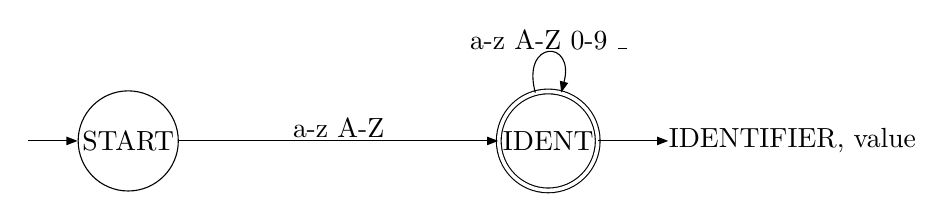
\begin{tikzpicture}[x=1in,y=1in,line width=0.4pt]
\node[draw,circle,fill=white,inner sep=1pt,minimum size=0.42in] (START) at (0.9,0.7) {START};
\node[draw,circle,fill=white,inner sep=1pt,minimum size=0.42in,double,double distance=1.3pt] (IDENT) at (3.0,0.7) {IDENT};
\draw[-{Triangle[length=4bp,width=3bp]}] (0.4,0.7) -- (START);
\node[inner sep=0pt,align=left,anchor=west] (IDENT-out) at (3.6,0.7) {\tok{IDENTIFIER, value}};
\draw[-{Triangle[length=4bp,width=3bp]}] (START) to[bend left=0] node[pos=0.5,above,inner sep=1pt,align=center] {\code{a-z} \code{A-Z}} (IDENT);
\path[-{Triangle[length=4bp,width=3bp]}] (IDENT) edge[loop above,min distance=7mm] node[above,inner sep=1pt,align=center] {\code{a-z} \code{A-Z} \code{0-9} \code{\_}} (IDENT);
\draw[-{Triangle[length=4bp,width=3bp]}] (IDENT) to[bend left=0] (IDENT-out.west);
\end{tikzpicture}
\end{adjustbox}
\caption{DFA for identifiers, keywords, type names, and bool literals.}
\label{fig:dfa-ident}
\end{figure}

\begin{table}[H]
\centering
\footnotesize
\begin{tabular}{@{}ll@{}}
\code{for} & \tok{FOR} \\
\code{do} & \tok{DO} \\
\code{until} & \tok{UNTIL} \\
\code{continue} & \tok{CONTINUE} \\
\code{function} & \tok{FUNCTION} \\
\code{return} & \tok{RETURN} \\
\code{if} & \tok{IF} \\
\code{else} & \tok{ELSE} \\
\code{elseif} & \tok{ELSEIF} \\
\code{caseof} & \tok{CASEOF} \\
\code{case} & \tok{CASE} \\
\code{default} & \tok{DEFAULT} \\
\code{and} & \tok{AND} \\
\code{or} & \tok{OR} \\
\code{not} & \tok{NOT} \\
\code{is} & \tok{IS} \\
\code{in} & \tok{IN} \\
\code{break} & \tok{BREAK} \\
\code{i64} \code{i32} \code{i16} \code{f64} \code{f32} \code{f16} \code{bool} & \tok{SCALAR, value} \\
\code{vector} & \tok{VECTOR} \\
\code{matrix} & \tok{MATRIX} \\
\code{string} & \tok{STRING} \\
\code{true} \code{false} & \tok{BOOL_LIT, value} \\
\end{tabular}
\caption{Keywords, type names, and bool literals, and the tokens the lookup after IDENT gives them.}
\label{tab:lookup}
\end{table}

\subsection{Punctuation}

A punctuation token is one of the characters \code{\symbol{123}}
\code{\symbol{125}} \code{(} \code{)} \code{[} \code{]} \code{;} \code{,}
\code{:}, or \code{->}, or \code{...}. A single character goes from
\code{START} straight to \code{OP\_DONE}. \code{->} goes through \code{MINUS},
and \code{...} goes through \code{DOT} and \code{DOT\_DOT}. These three states
are not accepting in this automaton, because \code{-} and \code{.} on their
own are not punctuation. \code{OP\_DONE} is accepting, and
Table~\ref{tab:punct} gives the token for each lexeme.

\begin{table}[H]
\centering
\footnotesize
\begin{tabular}{@{}ll@{}}
\code{\symbol{123}} & \tok{LBRACE} \\
\code{\symbol{125}} & \tok{RBRACE} \\
\code{(} & \tok{LPAREN} \\
\code{)} & \tok{RPAREN} \\
\code{[} & \tok{LBRACKET} \\
\code{]} & \tok{RBRACKET} \\
\code{;} & \tok{SEMICOLON} \\
\code{->} & \tok{ARROW} \\
\code{,} & \tok{COMMA} \\
\code{...} & \tok{ELLIPSIS} \\
\code{:} & \tok{COLON} \\
\end{tabular}
\caption{Punctuation lexemes and the tokens they give.}
\label{tab:punct}
\end{table}

\begin{figure}[H]
\centering
\begin{adjustbox}{max width=\linewidth,max height=0.4\textheight}
\begin{tikzpicture}[x=1in,y=1in,line width=0.4pt]
\node[draw,circle,fill=white,inner sep=1pt,minimum size=0.42in] (START) at (0.8,2.4) {START};
\node[draw,circle,fill=white,inner sep=1pt,minimum size=0.42in,double,double distance=1.3pt] (OP_DONE) at (4.3,2.4) {OP\_DONE};
\node[draw,circle,fill=white,inner sep=1pt,minimum size=0.42in] (MINUS) at (2.3,0.9) {MINUS};
\node[draw,circle,fill=white,inner sep=1pt,minimum size=0.42in] (DOT) at (2.1,3.9) {DOT};
\node[draw,circle,fill=white,inner sep=1pt,minimum size=0.42in] (DOT_DOT) at (3.4,3.9) {DOT\_DOT};
\draw[-{Triangle[length=4bp,width=3bp]}] (0.30000000000000004,2.4) -- (START);
\node[inner sep=0pt,align=left,anchor=west] (OP_DONE-out) at (5.0,2.4) {Table~\ref{tab:punct}};
\draw[-{Triangle[length=4bp,width=3bp]}] (START) to[bend left=0] node[pos=0.5,above,inner sep=1pt,align=center] {\code{(} \code{)} \code{,} \code{:} \code{;} \code{[} \code{]} \code{\symbol{123}} \code{\symbol{125}}} (OP_DONE);
\draw[-{Triangle[length=4bp,width=3bp]}] (START) to[bend left=0] node[pos=0.5,below left,inner sep=1pt,align=center] {\code{-}} (MINUS);
\draw[-{Triangle[length=4bp,width=3bp]}] (START) to[bend left=0] node[pos=0.5,above left,inner sep=1pt,align=center] {\code{.}} (DOT);
\draw[-{Triangle[length=4bp,width=3bp]}] (MINUS) to[bend left=0] node[pos=0.5,above left,inner sep=1pt,align=center] {\code{>}} (OP_DONE);
\draw[-{Triangle[length=4bp,width=3bp]}] (DOT) to[bend left=0] node[pos=0.5,above,inner sep=1pt,align=center] {\code{.}} (DOT_DOT);
\draw[-{Triangle[length=4bp,width=3bp]}] (DOT_DOT) to[bend left=0] node[pos=0.5,right,inner sep=1pt,align=center] {\code{.}} (OP_DONE);
\draw[-{Triangle[length=4bp,width=3bp]}] (OP_DONE) to[bend left=0] (OP_DONE-out.west);
\end{tikzpicture}
\end{adjustbox}
\caption{DFA for punctuation.}
\label{fig:dfa-punct}
\end{figure}

\subsection{Operators}
\label{sec:ops}

The operators are \code{+} \code{-} \code{*} \code{/} \code{\%}
\code{\textquotesingle{}}, the matrix operators \code{.*} and \code{./}, the
comparisons \code{<} \code{>} \code{<=} \code{>=}, and the assignments
\code{=} \code{+=} \code{-=} \code{*=} \code{/=}. \code{\%}
\code{\textquotesingle{}} \code{=} go from \code{START} straight to
\code{OP\_DONE}. \code{+} \code{*} \code{<} \code{>} go to \code{OP\_EQ},
\code{-} to \code{MINUS} and \code{/} to \code{SLASH}. These three states are
accepting, because each of those characters is an operator on its own, and
they continue to \code{OP\_DONE} on \code{=}. \code{DOT} is not accepting,
because \code{.} alone is not an operator. It continues to \code{OP\_DONE} on
\code{*} or \code{/}. The state a lexeme ends in does not fix its token, so
Table~\ref{tab:ops} gives the token for each lexeme.

There is no symbolic operator for equality or inequality, since these are
written with the words \code{is} and \code{is not}.

\begin{table}[H]
\centering
\footnotesize
\begin{tabular}{@{}ll@{}}
\code{+} \code{-} & \tok{PLUSMINUS, value} \\
\code{*} \code{/} \code{\%} & \tok{STAR_SLASH_MOD, value} \\
\code{\textquotesingle{}} & \tok{TRANSPOSE} \\
\code{.*} & \tok{DOT_STAR} \\
\code{./} & \tok{DOT_SLASH} \\
\code{<} & \tok{LESS} \\
\code{>} & \tok{GREATER} \\
\code{<=} & \tok{LESS_EQ} \\
\code{>=} & \tok{GREATER_EQ} \\
\code{=} \code{+=} \code{-=} \code{*=} \code{/=} & \tok{ASSIGNMENT, value} \\
\end{tabular}
\caption{Operator lexemes and the tokens they give.}
\label{tab:ops}
\end{table}

\begin{figure}[H]
\centering
\begin{adjustbox}{max width=\linewidth,max height=0.6\textheight}
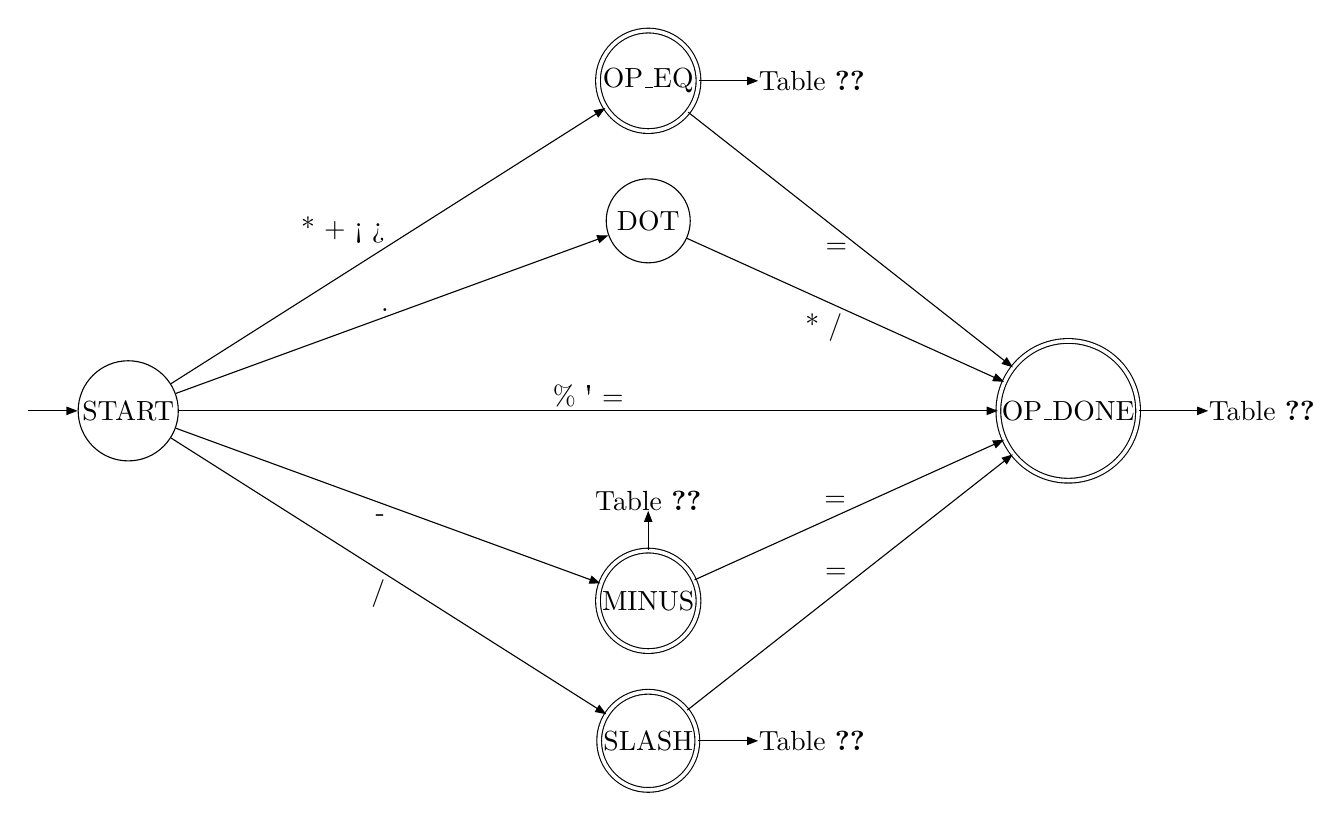
\begin{tikzpicture}[x=1in,y=1in,line width=0.4pt]
\node[draw,circle,fill=white,inner sep=1pt,minimum size=0.42in] (START) at (0.5,4.55) {START};
\node[draw,circle,fill=white,inner sep=1pt,minimum size=0.42in,double,double distance=1.3pt] (OP_DONE) at (5.2,4.55) {OP\_DONE};
\node[draw,circle,fill=white,inner sep=1pt,minimum size=0.42in,double,double distance=1.3pt] (MINUS) at (3.1,3.6) {MINUS};
\node[draw,circle,fill=white,inner sep=1pt,minimum size=0.42in,double,double distance=1.3pt] (OP_EQ) at (3.1,6.2) {OP\_EQ};
\node[draw,circle,fill=white,inner sep=1pt,minimum size=0.42in,double,double distance=1.3pt] (SLASH) at (3.1,2.9) {SLASH};
\node[draw,circle,fill=white,inner sep=1pt,minimum size=0.42in] (DOT) at (3.1,5.5) {DOT};
\draw[-{Triangle[length=4bp,width=3bp]}] (0.0,4.55) -- (START);
\node[inner sep=0pt,align=left,anchor=west] (OP_DONE-out) at (5.9,4.55) {Table~\ref{tab:ops}};
\node[inner sep=0pt,align=left,anchor=south] (MINUS-out) at (3.1,4.05) {Table~\ref{tab:ops}};
\node[inner sep=0pt,align=left,anchor=west] (OP_EQ-out) at (3.65,6.2) {Table~\ref{tab:ops}};
\node[inner sep=0pt,align=left,anchor=west] (SLASH-out) at (3.65,2.9) {Table~\ref{tab:ops}};
\draw[-{Triangle[length=4bp,width=3bp]}] (START) to[bend left=0] node[pos=0.5,above,inner sep=1pt,align=center] {\code{\%} \code{\textquotesingle{}} \code{=}} (OP_DONE);
\draw[-{Triangle[length=4bp,width=3bp]}] (START) to[bend left=0] node[pos=0.5,below left,inner sep=1pt,align=center] {\code{-}} (MINUS);
\draw[-{Triangle[length=4bp,width=3bp]}] (START) to[bend left=0] node[pos=0.5,above left,inner sep=1pt,align=center] {\code{*} \code{+} \code{<} \code{>}} (OP_EQ);
\draw[-{Triangle[length=4bp,width=3bp]}] (START) to[bend left=0] node[pos=0.5,below left,inner sep=1pt,align=center] {\code{/}} (SLASH);
\draw[-{Triangle[length=4bp,width=3bp]}] (START) to[bend left=0] node[pos=0.5,above left,inner sep=1pt,align=center] {\code{.}} (DOT);
\draw[-{Triangle[length=4bp,width=3bp]}] (MINUS) to[bend left=0] node[pos=0.5,above left,inner sep=1pt,align=center] {\code{=}} (OP_DONE);
\draw[-{Triangle[length=4bp,width=3bp]}] (OP_EQ) to[bend left=0] node[pos=0.5,below left,inner sep=1pt,align=center] {\code{=}} (OP_DONE);
\draw[-{Triangle[length=4bp,width=3bp]}] (SLASH) to[bend left=0] node[pos=0.5,above left,inner sep=1pt,align=center] {\code{=}} (OP_DONE);
\draw[-{Triangle[length=4bp,width=3bp]}] (DOT) to[bend left=0] node[pos=0.5,below left,inner sep=1pt,align=center] {\code{*} \code{/}} (OP_DONE);
\draw[-{Triangle[length=4bp,width=3bp]}] (OP_DONE) to[bend left=0] (OP_DONE-out.west);
\draw[-{Triangle[length=4bp,width=3bp]}] (MINUS) to[bend left=0] (MINUS-out.south);
\draw[-{Triangle[length=4bp,width=3bp]}] (OP_EQ) to[bend left=0] (OP_EQ-out.west);
\draw[-{Triangle[length=4bp,width=3bp]}] (SLASH) to[bend left=0] (SLASH-out.west);
\end{tikzpicture}
\end{adjustbox}
\caption{DFA for operators.}
\label{fig:dfa-ops}
\end{figure}

\subsection{Constants}

A constant is an int literal, a float literal, or a string literal. The bool
literals \code{true} and \code{false} are words, resolved through the
keyword lookup of Section~\ref{sec:ident} rather than through this DFA.

\begin{itemize}
    \item int literal: \code{[0-9]+}
    \item float literal: \code{[0-9]+\symbol{92}.[0-9]+} or
    \code{[0-9]+(\symbol{92}.[0-9]+)?[eE][+-]?[0-9]+}
    \item string literal: \code{\symbol{34}[\symbol{94}\symbol{34}\symbol{92}n]*\symbol{34}}
\end{itemize}

Digits are read in \code{INT}. A dot followed by digits leads through
\code{INT\_DOT} to \code{FLOAT}. An \code{e} or \code{E} after \code{INT} or
\code{FLOAT} leads to \code{EXP}, an optional sign to \code{EXP\_SIGN}, and
digits to \code{FLOAT\_EXP}. A quote starts \code{STR\_BODY}, which loops on
every character except a newline or a quote, and the closing quote reaches
\code{STR\_END}. \code{INT}, \code{FLOAT}, \code{FLOAT\_EXP} and
\code{STR\_END} are accepting.

\code{INT\_DOT}, \code{EXP}, and \code{EXP\_SIGN} are not accepting, so a
partial literal such as \code{1.} or \code{1e+} is not a number, and the lexer
falls back to the longest number that was complete, as described in
Section~\ref{sec:lexer-algorithm}. A float must have digits on both sides of
the dot, so \code{1.} and \code{.5} are lexical errors. A digit followed by a
letter other than \code{e} or \code{E} has no transition, so \code{12abc} is
read as the integer \code{12} followed by the identifier \code{abc}. There
are no escape sequences in strings, and a string cannot span lines: a newline
inside a string has no transition, so a string that is missing its closing
quote never reaches an accepting state and is reported as an error.

\begin{figure}[H]
\centering
\begin{adjustbox}{max width=\linewidth,max height=0.42\textheight}
\begin{tikzpicture}[x=1in,y=1in,line width=0.4pt]
\node[draw,circle,fill=white,inner sep=1pt,minimum size=0.42in] (START) at (0.6,3.1) {START};
\node[draw,circle,fill=white,inner sep=1pt,minimum size=0.42in,double,double distance=1.3pt] (INT) at (1.9,4.5) {INT};
\node[draw,circle,fill=white,inner sep=1pt,minimum size=0.42in] (INT_DOT) at (3.5,4.5) {INT\_DOT};
\node[draw,circle,fill=white,inner sep=1pt,minimum size=0.42in,double,double distance=1.3pt] (FLOAT) at (5.0,4.5) {FLOAT};
\node[draw,circle,fill=white,inner sep=1pt,minimum size=0.42in] (EXP) at (4.3,3.1) {EXP};
\node[draw,circle,fill=white,inner sep=1pt,minimum size=0.42in] (EXP_SIGN) at (3.1,1.9) {EXP\_SIGN};
\node[draw,circle,fill=white,inner sep=1pt,minimum size=0.42in,double,double distance=1.3pt] (FLOAT_EXP) at (5.0,1.9) {FLOAT\_EXP};
\node[draw,circle,fill=white,inner sep=1pt,minimum size=0.42in] (STR_BODY) at (1.9,0.9) {STR\_BODY};
\node[draw,circle,fill=white,inner sep=1pt,minimum size=0.42in,double,double distance=1.3pt] (STR_END) at (4.1,0.9) {STR\_END};
\draw[-{Triangle[length=4bp,width=3bp]}] (0.09999999999999998,3.1) -- (START);
\node[inner sep=0pt,align=left,anchor=south] (INT-out) at (1.9,5.05) {\tok{INT, value}};
\node[inner sep=0pt,align=left,anchor=south] (FLOAT-out) at (5.0,5.05) {\tok{FLOAT, value}};
\node[inner sep=0pt,align=left,anchor=north west] (FLOAT_EXP-out) at (5.2,1.3) {\tok{FLOAT, value}};
\node[inner sep=0pt,align=left,anchor=north west] (STR_END-out) at (4.25,0.4) {\tok{STRING_LIT, value}};
\draw[-{Triangle[length=4bp,width=3bp]}] (START) to[bend left=0] node[pos=0.5,above left,inner sep=1pt,align=center] {\code{0-9}} (INT);
\draw[-{Triangle[length=4bp,width=3bp]}] (START) to[bend left=0] node[pos=0.5,right,inner sep=1pt,align=center] {\code{\symbol{34}}} (STR_BODY);
\path[-{Triangle[length=4bp,width=3bp]}] (INT) edge[loop left,min distance=7mm] node[left,inner sep=1pt,align=center] {\code{0-9}} (INT);
\draw[-{Triangle[length=4bp,width=3bp]}] (INT) to[bend left=0] node[pos=0.5,above,inner sep=1pt,align=center] {\code{.}} (INT_DOT);
\draw[-{Triangle[length=4bp,width=3bp]}] (INT) to[bend left=0] node[pos=0.55,below left,inner sep=1pt,align=center] {\code{E} \code{e}} (EXP);
\draw[-{Triangle[length=4bp,width=3bp]}] (INT_DOT) to[bend left=0] node[pos=0.5,above,inner sep=1pt,align=center] {\code{0-9}} (FLOAT);
\path[-{Triangle[length=4bp,width=3bp]}] (FLOAT) edge[loop right,min distance=7mm] node[right,inner sep=1pt,align=center] {\code{0-9}} (FLOAT);
\draw[-{Triangle[length=4bp,width=3bp]}] (FLOAT) to[bend left=0] node[pos=0.5,right,inner sep=1pt,align=center] {\code{E} \code{e}} (EXP);
\draw[-{Triangle[length=4bp,width=3bp]}] (EXP) to[bend left=0] node[pos=0.5,below right,inner sep=1pt,align=center] {\code{+} \code{-}} (EXP_SIGN);
\draw[-{Triangle[length=4bp,width=3bp]}] (EXP) to[bend left=0] node[pos=0.5,right,inner sep=1pt,align=center] {\code{0-9}} (FLOAT_EXP);
\draw[-{Triangle[length=4bp,width=3bp]}] (EXP_SIGN) to[bend left=0] node[pos=0.5,above,inner sep=1pt,align=center] {\code{0-9}} (FLOAT_EXP);
\path[-{Triangle[length=4bp,width=3bp]}] (FLOAT_EXP) edge[loop right,min distance=7mm] node[right,inner sep=1pt,align=center] {\code{0-9}} (FLOAT_EXP);
\path[-{Triangle[length=4bp,width=3bp]}] (STR_BODY) edge[loop below,min distance=7mm] node[below,inner sep=1pt,align=center] {\code{any except \symbol{92}n \symbol{34}}} (STR_BODY);
\draw[-{Triangle[length=4bp,width=3bp]}] (STR_BODY) to[bend left=0] node[pos=0.5,above,inner sep=1pt,align=center] {\code{\symbol{34}}} (STR_END);
\draw[-{Triangle[length=4bp,width=3bp]}] (INT) to[bend left=0] (INT-out.south);
\draw[-{Triangle[length=4bp,width=3bp]}] (FLOAT) to[bend left=0] (FLOAT-out.south);
\draw[-{Triangle[length=4bp,width=3bp]}] (FLOAT_EXP) to[bend left=0] (FLOAT_EXP-out.north west);
\draw[-{Triangle[length=4bp,width=3bp]}] (STR_END) to[bend left=0] (STR_END-out.north west);
\end{tikzpicture}
\end{adjustbox}
\caption{DFA for constants.}
\label{fig:dfa-const}
\end{figure}

\subsection{Compiler Tokens}

The end of the input emits \tok{COMPILER_EOF}. The scanner
checks for the end of the input before it runs the DFA, so the code has no
state for it, and the transition goes straight from the start state to the
token. When the next character has no transition and no accepting state was passed, the DFA is in
\code{DEAD}, the error state of the code, and the text read so far is emitted
as \tok{COMPILER_ERROR}.

\begin{figure}[H]
\centering
\begin{adjustbox}{max width=\linewidth,max height=0.25\textheight}
\begin{tikzpicture}[x=1in,y=1in,line width=0.4pt]
\node[draw,circle,fill=white,inner sep=1pt,minimum size=0.42in] (START) at (0.9,1.8) {START};
\node[draw,circle,fill=white,inner sep=1pt,minimum size=0.42in] (DEAD) at (3.0,0.6) {DEAD};
\draw[-{Triangle[length=4bp,width=3bp]}] (0.4,1.8) -- (START);
\node[inner sep=0pt,align=left,anchor=west] (eof-out) at (3.4,1.8) {\tok{COMPILER_EOF}};
\node[inner sep=0pt,align=left,anchor=west] (DEAD-out) at (3.4,0.6) {\tok{COMPILER_ERROR}};
\draw[-{Triangle[length=4bp,width=3bp]}] (START) to[bend left=0] node[pos=0.5,above,inner sep=1pt,align=center] {\code{end of input}} (eof-out.west);
\draw[-{Triangle[length=4bp,width=3bp]}] (DEAD) to[bend left=0] (DEAD-out.west);
\end{tikzpicture}
\end{adjustbox}
\caption{DFA for the compiler tokens.}
\label{fig:dfa-compiler}
\end{figure}

\subsection{Skipped Input}

Skipped input is whitespace and comments. Whitespace is a run of the \code{WS}
and \code{NL} classes and stays in \code{WS}. A comment starts with \code{//}
and runs up to, but not including, the next newline, staying in
\code{COMMENT}. \code{WS} and \code{COMMENT} are accepting but emit no token.
\code{SLASH} is not accepting in this automaton, because a single \code{/} is
not skipped input: it is the division operator of Section~\ref{sec:ops}.

\begin{figure}[H]
\centering
\begin{adjustbox}{max width=\linewidth,max height=0.35\textheight}
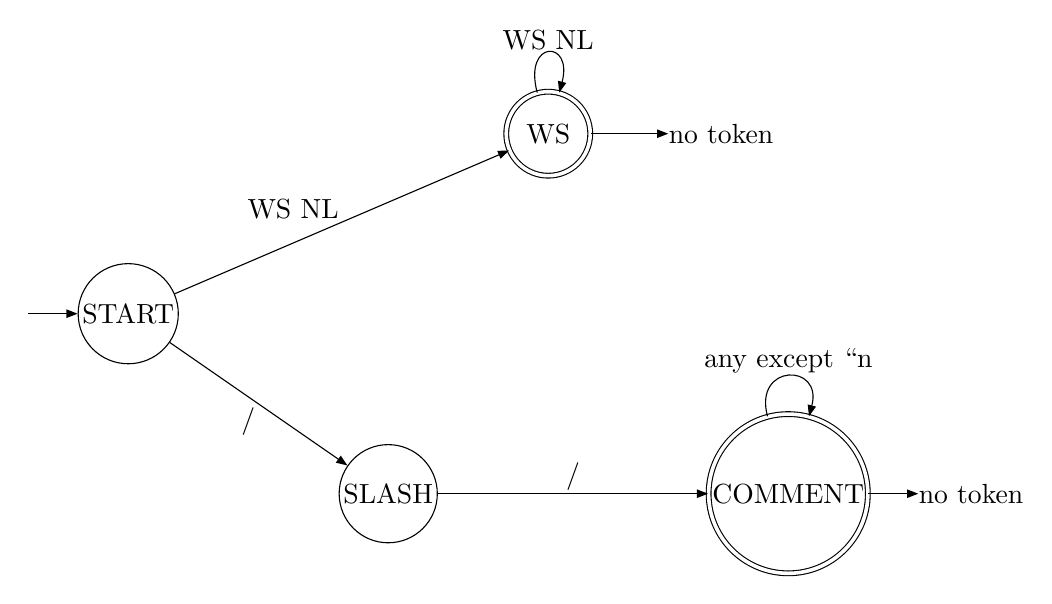
\begin{tikzpicture}[x=1in,y=1in,line width=0.4pt]
\node[draw,circle,fill=white,inner sep=1pt,minimum size=0.42in] (START) at (0.9,1.6) {START};
\node[draw,circle,fill=white,inner sep=1pt,minimum size=0.42in] (SLASH) at (2.2,0.7) {SLASH};
\node[draw,circle,fill=white,inner sep=1pt,minimum size=0.42in,double,double distance=1.3pt] (COMMENT) at (4.2,0.7) {COMMENT};
\node[draw,circle,fill=white,inner sep=1pt,minimum size=0.42in,double,double distance=1.3pt] (WS) at (3.0,2.5) {WS};
\draw[-{Triangle[length=4bp,width=3bp]}] (0.4,1.6) -- (START);
\node[inner sep=0pt,align=left,anchor=west] (COMMENT-out) at (4.85,0.7) {no token};
\node[inner sep=0pt,align=left,anchor=west] (WS-out) at (3.6,2.5) {no token};
\draw[-{Triangle[length=4bp,width=3bp]}] (START) to[bend left=0] node[pos=0.5,below left,inner sep=1pt,align=center] {\code{/}} (SLASH);
\draw[-{Triangle[length=4bp,width=3bp]}] (START) to[bend left=0] node[pos=0.5,above left,inner sep=1pt,align=center] {\code{WS} \code{NL}} (WS);
\draw[-{Triangle[length=4bp,width=3bp]}] (SLASH) to[bend left=0] node[pos=0.5,above,inner sep=1pt,align=center] {\code{/}} (COMMENT);
\path[-{Triangle[length=4bp,width=3bp]}] (COMMENT) edge[loop above,min distance=7mm] node[above,inner sep=1pt,align=center] {\code{any except \symbol{92}n}} (COMMENT);
\path[-{Triangle[length=4bp,width=3bp]}] (WS) edge[loop above,min distance=7mm] node[above,inner sep=1pt,align=center] {\code{WS} \code{NL}} (WS);
\draw[-{Triangle[length=4bp,width=3bp]}] (COMMENT) to[bend left=0] (COMMENT-out.west);
\draw[-{Triangle[length=4bp,width=3bp]}] (WS) to[bend left=0] (WS-out.west);
\end{tikzpicture}
\end{adjustbox}
\caption{DFA for whitespace and comments.}
\label{fig:dfa-skip}
\end{figure}

\subsection{The Merged DFA}

The classes are merged into one DFA, the one the lexer runs. Its states carry the
names the source gives them.

\begin{enumerate}
    \item A new start state has a transition for the first character of
    every class.
    \item Classes that share a prefix share states. Keywords, type names
    and identifiers are all read in IDENT, and operators and punctuation
    end in OP\_DONE, MINUS, OP\_EQ, SLASH, DOT and DOT\_DOT.
    \item A state that is accepting for one class stays accepting in the
    merged DFA, so MINUS and SLASH are accepting here.
    \item IDENT emits \tok{IDENTIFIER, value}, which
    Table~\ref{tab:lookup} replaces when the lexeme is a keyword or type
    name. OP\_EQ and OP\_DONE emit different tokens depending on the
    lexeme. The arrow from each of them names the tables that list them.
    \item The DFA runs until the next character has no transition. The
    token of the last accepting state passed is emitted, and if none was
    passed the consumed text is a \tok{COMPILER_ERROR}
    token. DEAD is not drawn: every missing transition leads to it.
\end{enumerate}

\begin{figure}[H]
\centering
\begin{adjustbox}{max width=\linewidth,max height=0.85\textheight}
\begin{tikzpicture}[x=1in,y=1in,line width=0.4pt]
\node[draw,circle,fill=white,inner sep=1pt,minimum size=0.42in] (START) at (0.6,7.1) {START};
\node[draw,circle,fill=white,inner sep=1pt,minimum size=0.42in,double,double distance=1.3pt] (IDENT) at (2.5,10.4) {IDENT};
\node[draw,circle,fill=white,inner sep=1pt,minimum size=0.42in,double,double distance=1.3pt] (INT) at (2.5,2.8) {INT};
\node[draw,circle,fill=white,inner sep=1pt,minimum size=0.42in] (INT_DOT) at (4.0,2.8) {INT\_DOT};
\node[draw,circle,fill=white,inner sep=1pt,minimum size=0.42in,double,double distance=1.3pt] (FLOAT) at (5.5,2.8) {FLOAT};
\node[draw,circle,fill=white,inner sep=1pt,minimum size=0.42in] (EXP) at (4.9,2.0) {EXP};
\node[draw,circle,fill=white,inner sep=1pt,minimum size=0.42in] (EXP_SIGN) at (3.6,1.2000000000000002) {EXP\_SIGN};
\node[draw,circle,fill=white,inner sep=1pt,minimum size=0.42in,double,double distance=1.3pt] (FLOAT_EXP) at (5.4,1.2000000000000002) {FLOAT\_EXP};
\node[draw,circle,fill=white,inner sep=1pt,minimum size=0.42in,double,double distance=1.3pt] (OP_DONE) at (4.9,7.1) {OP\_DONE};
\node[draw,circle,fill=white,inner sep=1pt,minimum size=0.42in,double,double distance=1.3pt] (MINUS) at (2.5,6.1) {MINUS};
\node[draw,circle,fill=white,inner sep=1pt,minimum size=0.42in,double,double distance=1.3pt] (OP_EQ) at (2.5,8.0) {OP\_EQ};
\node[draw,circle,fill=white,inner sep=1pt,minimum size=0.42in,double,double distance=1.3pt] (SLASH) at (2.5,5.1) {SLASH};
\node[draw,circle,fill=white,inner sep=1pt,minimum size=0.42in,double,double distance=1.3pt] (COMMENT) at (2.5,4.1) {COMMENT};
\node[draw,circle,fill=white,inner sep=1pt,minimum size=0.42in] (DOT) at (2.5,9.100000000000001) {DOT};
\node[draw,circle,fill=white,inner sep=1pt,minimum size=0.42in] (DOT_DOT) at (4.0,9.55) {DOT\_DOT};
\node[draw,circle,fill=white,inner sep=1pt,minimum size=0.42in] (STR_BODY) at (2.5,11.700000000000001) {STR\_BODY};
\node[draw,circle,fill=white,inner sep=1pt,minimum size=0.42in,double,double distance=1.3pt] (STR_END) at (4.6,11.700000000000001) {STR\_END};
\node[draw,circle,fill=white,inner sep=1pt,minimum size=0.42in,double,double distance=1.3pt] (WS) at (2.5,13.0) {WS};
\draw[-{Triangle[length=4bp,width=3bp]}] (0.09999999999999998,7.1) -- (START);
\node[inner sep=0pt,align=left,anchor=west] (IDENT-out) at (3.15,10.4) {\tok{IDENTIFIER, value}};
\node[inner sep=0pt,align=left,anchor=north] (INT-out) at (1.6,2.3) {\tok{INT, value}};
\node[inner sep=0pt,align=left,anchor=south] (FLOAT-out) at (5.5,3.3499999999999996) {\tok{FLOAT, value}};
\node[inner sep=0pt,align=left,anchor=north] (FLOAT_EXP-out) at (5.4,0.65) {\tok{FLOAT, value}};
\node[inner sep=0pt,align=left,anchor=west] (OP_DONE-out) at (5.35,7.1) {Tables~\ref{tab:punct} and~\ref{tab:ops}};
\node[inner sep=0pt,align=left,anchor=north] (MINUS-out) at (2.5,5.7) {\tok{PLUSMINUS, value}};
\node[inner sep=0pt,align=left,anchor=south] (OP_EQ-out) at (2.5,8.35) {Table~\ref{tab:ops}};
\node[inner sep=0pt,align=left,anchor=west] (SLASH-out) at (2.9,4.75) {\tok{STAR_SLASH_MOD, value}};
\node[inner sep=0pt,align=left,anchor=west] (COMMENT-out) at (3.1,4.1) {no token};
\node[inner sep=0pt,align=left,anchor=north] (STR_END-out) at (4.6,11.25) {\tok{STRING_LIT, value}};
\node[inner sep=0pt,align=left,anchor=west] (WS-out) at (3.1,13.0) {no token};
\draw[-{Triangle[length=4bp,width=3bp]}] (IDENT) to[bend left=0] (IDENT-out.west);
\draw[-{Triangle[length=4bp,width=3bp]}] (INT) to[bend left=0] (INT-out.north);
\draw[-{Triangle[length=4bp,width=3bp]}] (FLOAT) to[bend left=0] (FLOAT-out.south);
\draw[-{Triangle[length=4bp,width=3bp]}] (FLOAT_EXP) to[bend left=0] (FLOAT_EXP-out.north);
\draw[-{Triangle[length=4bp,width=3bp]}] (OP_DONE) to[bend left=0] (OP_DONE-out.west);
\draw[-{Triangle[length=4bp,width=3bp]}] (MINUS) to[bend left=0] (MINUS-out.north);
\draw[-{Triangle[length=4bp,width=3bp]}] (OP_EQ) to[bend left=0] (OP_EQ-out.south);
\draw[-{Triangle[length=4bp,width=3bp]}] (SLASH) to[bend left=0] (SLASH-out.west);
\draw[-{Triangle[length=4bp,width=3bp]}] (COMMENT) to[bend left=0] (COMMENT-out.west);
\draw[-{Triangle[length=4bp,width=3bp]}] (STR_END) to[bend left=0] (STR_END-out.north);
\draw[-{Triangle[length=4bp,width=3bp]}] (WS) to[bend left=0] (WS-out.west);
\draw[-{Triangle[length=4bp,width=3bp]}] (START) |- node[pos=0.817,above,inner sep=1pt,align=center] {\code{LETTER} \code{EXP}} (IDENT);
\draw[-{Triangle[length=4bp,width=3bp]}] (START) |- node[pos=0.847,above,inner sep=1pt,align=center] {\code{DIGIT}} (INT);
\draw[-{Triangle[length=4bp,width=3bp]}] (START) to[bend left=0] node[pos=0.5,above,inner sep=1pt,align=center] {\code{EQ} \code{SIMPLE}} (OP_DONE);
\draw[-{Triangle[length=4bp,width=3bp]}] (START) |- node[pos=0.672,above,inner sep=1pt,align=center] {\code{MINUS}} (MINUS);
\draw[-{Triangle[length=4bp,width=3bp]}] (START) |- node[pos=0.661,above,inner sep=1pt,align=center] {\code{PLUS} \code{STAR} \code{LT} \code{GT}} (OP_EQ);
\draw[-{Triangle[length=4bp,width=3bp]}] (START) |- node[pos=0.756,above,inner sep=1pt,align=center] {\code{SLASH}} (SLASH);
\draw[-{Triangle[length=4bp,width=3bp]}] (START) |- node[pos=0.756,above,inner sep=1pt,align=center] {\code{DOT}} (DOT);
\draw[-{Triangle[length=4bp,width=3bp]}] (START) |- node[pos=0.854,above,inner sep=1pt,align=center] {\code{QUOTE}} (STR_BODY);
\draw[-{Triangle[length=4bp,width=3bp]}] (START) |- node[pos=0.878,above,inner sep=1pt,align=center] {\code{WS} \code{NL}} (WS);
\path[-{Triangle[length=4bp,width=3bp]}] (IDENT) edge[loop above,min distance=7mm] node[above,inner sep=1pt,align=center] {\code{LETTER} \code{EXP} \code{DIGIT} \code{\_}} (IDENT);
\path[-{Triangle[length=4bp,width=3bp]}] (INT) edge[loop above,min distance=7mm] node[above,inner sep=1pt,align=center] {\code{DIGIT}} (INT);
\draw[-{Triangle[length=4bp,width=3bp]}] (INT) to[bend left=0] node[pos=0.5,above,inner sep=1pt,align=center] {\code{DOT}} (INT_DOT);
\draw[-{Triangle[length=4bp,width=3bp]}] (INT) to[bend left=0] node[pos=0.5,below left,inner sep=1pt,align=center] {\code{EXP}} (EXP);
\draw[-{Triangle[length=4bp,width=3bp]}] (INT_DOT) to[bend left=0] node[pos=0.5,above,inner sep=1pt,align=center] {\code{DIGIT}} (FLOAT);
\path[-{Triangle[length=4bp,width=3bp]}] (FLOAT) edge[loop right,min distance=7mm] node[right,inner sep=1pt,align=center] {\code{DIGIT}} (FLOAT);
\draw[-{Triangle[length=4bp,width=3bp]}] (FLOAT) to[bend left=0] node[pos=0.5,right,inner sep=1pt,align=center] {\code{EXP}} (EXP);
\draw[-{Triangle[length=4bp,width=3bp]}] (EXP) to[bend left=0] node[pos=0.5,above left,inner sep=1pt,align=center] {\code{PLUS} \code{MINUS}} (EXP_SIGN);
\draw[-{Triangle[length=4bp,width=3bp]}] (EXP) to[bend left=0] node[pos=0.5,right,inner sep=1pt,align=center] {\code{DIGIT}} (FLOAT_EXP);
\draw[-{Triangle[length=4bp,width=3bp]}] (EXP_SIGN) to[bend left=0] node[pos=0.5,above,inner sep=1pt,align=center] {\code{DIGIT}} (FLOAT_EXP);
\path[-{Triangle[length=4bp,width=3bp]}] (FLOAT_EXP) edge[loop right,min distance=7mm] node[right,inner sep=1pt,align=center] {\code{DIGIT}} (FLOAT_EXP);
\draw[-{Triangle[length=4bp,width=3bp]}] (MINUS) -| node[pos=0.353,above,inner sep=1pt,align=center] {\code{GT} \code{EQ}} (OP_DONE);
\draw[-{Triangle[length=4bp,width=3bp]}] (OP_EQ) -| node[pos=0.364,above,inner sep=1pt,align=center] {\code{EQ}} (OP_DONE);
\draw[-{Triangle[length=4bp,width=3bp]}] (SLASH) -| node[pos=0.273,above,inner sep=1pt,align=center] {\code{EQ}} (OP_DONE);
\draw[-{Triangle[length=4bp,width=3bp]}] (SLASH) to[bend left=0] node[pos=0.5,left,inner sep=1pt,align=center] {\code{SLASH}} (COMMENT);
\path[-{Triangle[length=4bp,width=3bp]}] (COMMENT) edge[loop left,min distance=7mm] node[left,inner sep=1pt,align=center] {\code{any except NL}} (COMMENT);
\draw[-{Triangle[length=4bp,width=3bp]}] (DOT) -| node[pos=0.273,below,inner sep=1pt,align=center] {\code{STAR} \code{SLASH}} (OP_DONE);
\draw[-{Triangle[length=4bp,width=3bp]}] (DOT) to[bend left=0] node[pos=0.5,above left,inner sep=1pt,align=center] {\code{DOT}} (DOT_DOT);
\draw[-{Triangle[length=4bp,width=3bp]}] (DOT_DOT) -| node[pos=0.134,above,inner sep=1pt,align=center] {\code{DOT}} (OP_DONE);
\path[-{Triangle[length=4bp,width=3bp]}] (STR_BODY) edge[loop above,min distance=7mm] node[above,inner sep=1pt,align=center] {\code{any except NL QUOTE}} (STR_BODY);
\draw[-{Triangle[length=4bp,width=3bp]}] (STR_BODY) to[bend left=0] node[pos=0.5,above,inner sep=1pt,align=center] {\code{QUOTE}} (STR_END);
\path[-{Triangle[length=4bp,width=3bp]}] (WS) edge[loop above,min distance=7mm] node[above,inner sep=1pt,align=center] {\code{WS} \code{NL}} (WS);
\end{tikzpicture}
\end{adjustbox}
\caption{The merged DFA of the lexer.}
\label{fig:dfa-merged}
\end{figure}

\section{The Lexical Analyzer Algorithm}
\label{sec:lexer-algorithm}

The scanner exposes a single operation, \code{next}, which returns the next
token each time it is called. It keeps the source text, the current position,
and the current line and column, both counted from 1. The reference
implementation is a C++ program.

\subsection{Maximal Munch}

Each call to \code{next} starts at the current position and walks the
transition table for as long as a transition exists. Whenever it enters an
accepting state it records that state and the position reached. When it
reaches the dead state, or the end of the input, it rewinds to the last
recorded position. This is the longest match rule: the lexer always takes the
longest prefix that forms a token \cite{aho2006compilers}. The rewinding is
what allows one automaton to handle lexemes that share a prefix.

The text \code{0...2} shows this. The lexer reads \code{0}, which is accepting,
and then a dot, which moves to \code{INT\_DOT}. The next dot has no transition
from \code{INT\_DOT}, so the lexer rewinds to the \code{0} and emits it as an
integer literal. Scanning resumes at the first dot, which reaches
\code{OP\_DONE} after three dots and emits the ellipsis, and then \code{2} is
scanned on its own. In the same way, \code{1e+;} is scanned as the integer
\code{1}, the identifier \code{e}, and the operator \code{+}, because
\code{EXP} and \code{EXP\_SIGN} are not accepting.

\subsection{The Scanning Loop}

Listing~\ref{lst:scan-loop} shows the body of \code{next}. The character class
mapping is written \code{classOf}, and \code{advance} moves the position
forward while updating the line and column. The two lookup tables described
earlier are used through two functions. The function \code{lookupKeyword}
handles words, and \code{lookupOperator} handles operators.

\begin{lstlisting}[style=pseudocode, float=tbp,
    caption={The scanning loop of the lexer.}, label=lst:scan-loop]
function next():
    loop:
        if pos >= length(src):
            return Token(COMPILER_EOF)

        start <- pos
        state <- START
        lastAccept <- DEAD
        lastEnd <- start
        cur <- start

        while cur < length(src):
            nxt <- TRANSITION[state][classOf(src[cur])]
            if nxt is DEAD: break
            state <- nxt
            cur <- cur + 1
            if ACTION[state] is not NONE:
                lastAccept <- state
                lastEnd <- cur

        if lastAccept is DEAD:
            end <- start + 1 if cur = start else cur
            lexeme <- src[start .. end)
            advance(end - start)
            return Token(COMPILER_ERROR, lexeme)

        lexeme <- src[start .. lastEnd)
        advance(lastEnd - start)

        switch ACTION[lastAccept]:
            WORD:    type <- lookupKeyword(lexeme)
            INT:     type <- INT
            FLOAT:   type <- FLOAT
            OP:      type <- lookupOperator(lexeme)
            STRING:  type <- STRING_LIT
            SKIP:    continue    // scan again
        return Token(type, lexeme)
\end{lstlisting}

Each token also records the line and column where it started, which are taken
before the position moves.

\subsection{Resolving the Token}

The action of the last accepting state says how to name the lexeme. A word is
looked up in the keyword table, which also holds the type names and the bool
literals, and falls back to an identifier. An operator or punctuator is looked
up in the operator table. Integer literals, float literals, and string literals 
are named directly by their state. Whitespace and comments are skipped, and the 
loop starts again from the new position, so \code{next} never returns them.

\subsection{Errors}

If the walk never reached an accepting state, the text it consumed becomes the
lexeme of an error token, and at least one character is consumed so that
scanning always makes progress. The lexer then reports the lexeme on the
standard error stream, together with its line and column, the source line
it came from, and a marker under the lexeme, and scanning resumes right
after it. One run therefore reports every lexical error in a file.
Table~\ref{tab:lexer-errors} shows how some invalid inputs are reported.

\begin{table}[tbp]
\centering
\small
\renewcommand{\arraystretch}{1.1}
\begin{tabular}{@{}ll@{}}
\toprule
\textbf{Input} & \textbf{Reported lexeme} \\
\midrule
\code{\_hidden} & \code{\_} \\
\code{1.} & \code{.} \\
\code{.5} & \code{.} \\
\code{1.5.2} & \code{.} \\
\code{3..4} & \code{..} \\
\code{"unterminated} & \code{"unterminated} \\
\code{!=} & \code{!} \\
\code{a @ b} & \code{@} \\
\bottomrule
\end{tabular}
\caption{Examples of lexical errors.}
\label{tab:lexer-errors}
\end{table}

\subsection{Token Output}

The lexer writes one token per line in the form \code{<TYPE, value>}, ending
with the end of file token. Only some tokens have a value part: identifiers,
scalar type names, bool, integer, float, and string literals, the arithmetic
operators, and the assignment operators. These are the tokens whose Values
column is filled in Table~\ref{tab:token-set}. Every other token is written
with an empty value part, for example \code{<LBRACE,>}.

\subsection{Sample Runs}

To see the algorithm at work, we run the lexer on three statements. For each
lexeme, the tables list the states the automaton visits, starting from
\code{START}, followed by the lookup that names the lexeme when there is one,
and ending in the token that comes out. The whitespace between lexemes
takes the automaton through \code{WS}, which is skipped, so it does not appear
in the tables. After the last lexeme of the input, the lexer returns the end of
file token, \code{<COMPILER\_EOF,>}, which is also left out.

\medskip
\noindent\begin{minipage}{\textwidth}
\noindent\textbf{Statement 1.} The first statement declares a variable. Every lexeme is either a word, a number, or a single character.

\begin{lstlisting}
i32 count = 10;
\end{lstlisting}

\begin{center}
\footnotesize
\renewcommand{\arraystretch}{1.1}
\setlength{\tabcolsep}{4pt}
\begin{tabular}{@{}l>{\raggedright\arraybackslash}p{370pt}@{}}
\toprule
\textbf{Lexeme} & \textbf{States visited, lookup, and token} \\
\midrule
\code{i32} & \stok{START} $\to$ \stok{IDENT} $\to$ \stok{IDENT} $\to$ \stok{IDENT} $\to$ lookup(keyword table) $\to$ \tok{SCALAR, i32} \\
\code{count} & \stok{START} $\to$ \stok{IDENT} $\to$ \stok{IDENT} $\to$ \stok{IDENT} $\to$ \stok{IDENT} $\to$ \stok{IDENT} $\to$ lookup(keyword table) $\to$ \tok{IDENTIFIER, count} \\
\code{=} & \stok{START} $\to$ \stok{OP_DONE} $\to$ lookup(operator table) $\to$ \tok{ASSIGNMENT, =} \\
\code{10} & \stok{START} $\to$ \stok{INT} $\to$ \stok{INT} $\to$ \tok{INT, 10} \\
\code{;} & \stok{START} $\to$ \stok{OP_DONE} $\to$ lookup(operator table) $\to$ \tok{SEMICOLON} \\
\bottomrule
\end{tabular}
\end{center}
\end{minipage}
\medskip


\medskip
\noindent\begin{minipage}{\textwidth}
\noindent\textbf{Statement 2.} The second statement has a float with an exponent, and a matrix operator that is written without spaces around it.

\begin{lstlisting}
f32 y = 2.5e-3 + a.*b;
\end{lstlisting}

\begin{center}
\footnotesize
\renewcommand{\arraystretch}{1.1}
\setlength{\tabcolsep}{4pt}
\begin{tabular}{@{}l>{\raggedright\arraybackslash}p{370pt}@{}}
\toprule
\textbf{Lexeme} & \textbf{States visited, lookup, and token} \\
\midrule
\code{f32} & \stok{START} $\to$ \stok{IDENT} $\to$ \stok{IDENT} $\to$ \stok{IDENT} $\to$ lookup(keyword table) $\to$ \tok{SCALAR, f32} \\
\code{y} & \stok{START} $\to$ \stok{IDENT} $\to$ lookup(keyword table) $\to$ \tok{IDENTIFIER, y} \\
\code{=} & \stok{START} $\to$ \stok{OP_DONE} $\to$ lookup(operator table) $\to$ \tok{ASSIGNMENT, =} \\
\code{2.5e-3} & \stok{START} $\to$ \stok{INT} $\to$ \stok{INT_DOT} $\to$ \stok{FLOAT} $\to$ \stok{EXP} $\to$ \stok{EXP_SIGN} $\to$ \stok{FLOAT_EXP} $\to$ \tok{FLOAT, 2.5e-3} \\
\code{+} & \stok{START} $\to$ \stok{OP_EQ} $\to$ lookup(operator table) $\to$ \tok{PLUSMINUS, +} \\
\code{a} & \stok{START} $\to$ \stok{IDENT} $\to$ lookup(keyword table) $\to$ \tok{IDENTIFIER, a} \\
\code{.*} & \stok{START} $\to$ \stok{DOT} $\to$ \stok{OP_DONE} $\to$ lookup(operator table) $\to$ \tok{DOT_STAR} \\
\code{b} & \stok{START} $\to$ \stok{IDENT} $\to$ lookup(keyword table) $\to$ \tok{IDENTIFIER, b} \\
\code{;} & \stok{START} $\to$ \stok{OP_DONE} $\to$ lookup(operator table) $\to$ \tok{SEMICOLON} \\
\bottomrule
\end{tabular}
\end{center}
\end{minipage}
\medskip


\medskip
\noindent\begin{minipage}{\textwidth}
\noindent\textbf{Statement 3.} The third statement is the range loop, and the range \code{1...5} is the case where the lexer has to rewind.

\begin{lstlisting}
for (i32 i = 1...5) {
\end{lstlisting}

\begin{center}
\footnotesize
\renewcommand{\arraystretch}{1.1}
\setlength{\tabcolsep}{4pt}
\begin{tabular}{@{}l>{\raggedright\arraybackslash}p{370pt}@{}}
\toprule
\textbf{Lexeme} & \textbf{States visited, lookup, and token} \\
\midrule
\code{for} & \stok{START} $\to$ \stok{IDENT} $\to$ \stok{IDENT} $\to$ \stok{IDENT} $\to$ lookup(keyword table) $\to$ \tok{FOR} \\
\code{(} & \stok{START} $\to$ \stok{OP_DONE} $\to$ lookup(operator table) $\to$ \tok{LPAREN} \\
\code{i32} & \stok{START} $\to$ \stok{IDENT} $\to$ \stok{IDENT} $\to$ \stok{IDENT} $\to$ lookup(keyword table) $\to$ \tok{SCALAR, i32} \\
\code{i} & \stok{START} $\to$ \stok{IDENT} $\to$ lookup(keyword table) $\to$ \tok{IDENTIFIER, i} \\
\code{=} & \stok{START} $\to$ \stok{OP_DONE} $\to$ lookup(operator table) $\to$ \tok{ASSIGNMENT, =} \\
\code{1} & \stok{START} $\to$ \stok{INT} $\to$ \stok{INT_DOT} \textit{(no move on the next dot, rewind to \stok{INT})} $\to$ \tok{INT, 1} \\
\code{...} & \stok{START} $\to$ \stok{DOT} $\to$ \stok{DOT_DOT} $\to$ \stok{OP_DONE} $\to$ lookup(operator table) $\to$ \tok{ELLIPSIS} \\
\code{5} & \stok{START} $\to$ \stok{INT} $\to$ \tok{INT, 5} \\
\code{)} & \stok{START} $\to$ \stok{OP_DONE} $\to$ lookup(operator table) $\to$ \tok{RPAREN} \\
\code{\{} & \stok{START} $\to$ \stok{OP_DONE} $\to$ lookup(operator table) $\to$ \tok{LBRACE} \\
\bottomrule
\end{tabular}
\end{center}
\end{minipage}
\medskip


\medskip
\noindent In the first two runs, every lexeme is accepted at the last state it reaches,
and the lexer never has to go back. The word \code{i32} ends in \code{IDENT},
and the keyword table turns it into a type token. The float \code{2.5e-3} is
the longest path in the automaton, and it passes through three states that
are not accepting. In the third run, the \code{1} is followed by a dot, which
moves the automaton to \code{INT\_DOT}. The next character is another dot, which
has no transition there, so the lexer goes back to the last accepting state,
which was reached after the \code{1}, and returns the integer. The scan for the
next token then starts at the first dot, and reads all three of them.

\section{Lexers in the Real World}
\label{sec:lexers-real-world}

The lexer of OctaC is deliberately small. This section looks at how lexers
are built in practice, what they handle that ours does not, and which
simplifications we made.

\subsection{Lexer Generators}

Many lexers are produced by a generator such as Lex \cite{lesk1975lex} or its
successor Flex \cite{flex-manual}. The programmer writes a list of regular
expressions, each with an action. The generator converts them into a
deterministic finite automaton and emits a table-driven scanner
\cite{aho2006compilers}. Two rules resolve conflicts between patterns: the
longest match wins, and among patterns that match the same length, the one
listed first wins \cite{lesk1975lex,flex-manual}. Our scanner follows the
longest match rule. The second rule is not needed, because keywords are not
patterns of their own.

Flex recommends matching identifiers with one pattern and looking keywords up
in a table, instead of writing a pattern for each keyword
\cite{flex-manual}, which is what OctaC does. Flex also warns that a scanner
which has to back up over several characters is slower, and offers ways to
find and remove such cases \cite{flex-manual}. Our scanner backs up too, as the
run of \code{1...5} shows, but only over a few characters. Generators also
compress their tables \cite{aho2006compilers}. Ours has 19 states and 17
character classes, which is small enough to be stored as it is.

\subsection{Hand-Written Lexers}

Many production compilers do not use a generator. The lexer of the GNU C
preprocessor is coded by hand and is not implemented as a state machine
\cite{gcc-cppinternals}, and Clang has a hand-written lexer that scans the
source buffer directly \cite{clang-internals}. A hand-written lexer gives full
control over the speed of the scanner, the quality of error messages, and the
handling of features that regular expressions describe poorly. The lexer of
OctaC sits between the two approaches. The table is written by hand, but the
scanning loop is the same one that a generator would emit.

\subsection{What Real Lexers Handle}

Lexers for established languages deal with many things that OctaC leaves out:

\begin{itemize}
    \item \textbf{Richer literals.} Numbers may be written in hexadecimal,
    octal, or binary, with digit separators and type suffixes. Strings have
    escape sequences, raw forms, and may span lines \cite{rust-reference}.
    \item \textbf{More kinds of comments.} Block comments exist in many
    languages, and in Rust they can be nested \cite{rust-reference}.
    \item \textbf{Unicode.} Identifiers may contain letters from any script,
    following the rules of Unicode Standard Annex 31
    \cite{unicode-uax31,python-reference}.
    \item \textbf{Layout.} Python's lexer produces indent and dedent tokens
    from the indentation of each line \cite{python-reference}. The lexer of
    Go inserts semicolons at the ends of lines by a fixed rule, so programs
    can leave most of them out \cite{go-spec}.
    \item \textbf{Preprocessing.} A C lexer works together with the
    preprocessor, which handles macros and file inclusion
    \cite{gcc-cppinternals}.
\end{itemize}

\subsection{Simplifications in OctaC}

Table~\ref{tab:lexer-simplifications} summarizes the differences. Each of the
simplifications keeps the automaton small, and each could be lifted later by
adding states and character classes to the table.

\begin{table}[tbp]
\centering
\small
\renewcommand{\arraystretch}{1.15}
\begin{tabular}{@{}>{\raggedright\arraybackslash}p{62pt}>{\raggedright\arraybackslash}p{190pt}>{\raggedright\arraybackslash}p{180pt}@{}}
\toprule
\textbf{Concern} & \textbf{Real-world lexers} & \textbf{OctaC} \\
\midrule
Construction & Generated from regular expressions, or written by hand \cite{flex-manual,clang-internals} & One hand-written transition table \\
Characters & Unicode text, usually as UTF-8 & Bytes; anything outside the listed classes is an error \\
Identifiers & Unicode letters allowed \cite{unicode-uax31} & ASCII letters, digits, and underscores, starting with a letter \\
Numbers & Hexadecimal, binary, separators, suffixes \cite{rust-reference} & Decimal integers and floats, with an optional exponent \\
Strings & Escapes, raw strings, multiple lines \cite{rust-reference} & None of these: one line, no escapes \\
Comments & Block comments, sometimes nested \cite{rust-reference} & Line comments with \code{//} only \\
Layout & Indentation tokens, semicolon insertion \cite{python-reference,go-spec} & Whitespace is not significant, and semicolons are explicit \\
Preprocessing & Macros and file inclusion \cite{gcc-cppinternals} & None \\
Keywords & Table lookup after matching an identifier \cite{flex-manual} & Same \\
Errors & Diagnostics with recovery & Error token, a diagnostic, and scanning resumes \\
Input & Streamed through a buffer & The whole file is read into memory \\
\bottomrule
\end{tabular}
\caption{Real-world lexers compared with the OctaC lexer.}
\label{tab:lexer-simplifications}
\end{table}

% p1-chp03-parser.tex

\chapter{Syntax Analysis and the Parser}
\label{chp:parser}

The parser is the second phase of a compiler. It reads the token stream
produced by the lexer and builds a parse tree according to the grammar,
checking along the way that the tokens form a program that the grammar
allows. This chapter gives OctaC's grammar, in LL(1) form, and describes
the recursive descent parser built from it. The parser
chooses a production from one token of lookahead, builds the tree as it
goes, and recovers when it hits a syntax error. The source code of the
parser is available at:
\url{https://github.com/Octa-C/compiler/tree/main/parser}

\section{Grammar Theory}
\label{sec:grammar-theory}

\subsection{Left-Recursive Grammars}

A grammar is left recursive if it has a nonterminal $A$ with a production
of the form $A \to A\alpha \mid \beta$, where $\beta$ does not itself start
with $A$. Such a rule can never be used by a recursive descent parser: the
function for $A$ would call itself before reading any token, and never
terminate \cite{aho2006compilers}. The standard fix moves the recursive
part into a new nonterminal $A'$ that follows the non-recursive
alternative:
\begin{center}
$A \to \beta A'$ \qquad $A' \to \alpha A' \mid \varepsilon$
\end{center}
This produces the same language as the original rule, since $A$ is still
$\beta$ followed by zero or more repetitions of $\alpha$, just written so
that the recursion is no longer on the left \cite{aho2006compilers}. A sum
written as a left-recursive grammar, for example,
\begin{center}
$G \to G \mathbin{+} T \mid T$
\end{center}
rewrites the same way, with $\beta$ as $T$ and $\alpha$ as $\mathbin{+}\, T$:
\begin{center}
$G \to T G'$ \qquad $G' \to \mathbin{+}\, T G' \mid \varepsilon$
\end{center}

A grammar also needs left factoring when two productions of the same
nonterminal share a prefix, so that the parser cannot tell them apart from
the first token. Two productions of the form $A \to \alpha\beta_1 \mid
\alpha\beta_2$ can be rewritten by factoring the shared prefix out into a
new nonterminal, deferring the choice between $\beta_1$ and $\beta_2$ until
after $\alpha$ has been read \cite{aho2006compilers}:
\begin{center}
$A \to \alpha A'$ \qquad $A' \to \beta_1 \mid \beta_2$
\end{center}
A statement grammar with three productions that all start with an
identifier,
\begin{center}
$S \to \texttt{id}\ \texttt{=}\ \texttt{number} \mid \texttt{id}\,\texttt{(}\texttt{)}
\mid \texttt{id}\,\texttt{[}\texttt{]}$
\end{center}
needs exactly this treatment: factoring \texttt{id} out of all three gives
$S \to \texttt{id}\,S'$, with $S'$ then choosing between the three endings:
\begin{center}
$S \to \texttt{id}\,S'$ \qquad
$S' \to \texttt{=}\ \texttt{number} \mid \texttt{(}\texttt{)} \mid \texttt{[}\texttt{]}$
\end{center}

\subsection{LL(k) Grammars}

Eliminating left recursion and left factoring, as above, is not just a fix
for recursive descent specifically: it is what turns a grammar into a
grammar of a well known class. A parser that reads its input left to right
and builds a leftmost derivation, choosing a production for each
nonterminal from the next $k$ tokens of input without ever backtracking, is
called an LL($k$) parser, and a grammar it can parse this way is an LL($k$)
grammar \cite{aho2006compilers}. The first L is the direction the input is
read, the second is the kind of derivation built, and $k$ is how far ahead
the parser is allowed to look.

A grammar fails to be LL(1) when some nonterminal has two productions whose
possible starting tokens overlap, since then one token of lookahead is not
enough to choose between them \cite{aho2006compilers}. That is precisely
the problem left recursion and shared prefixes cause, and precisely what
eliminating them fixes. LL(1), with a single token of lookahead, is the
common case, and it is exactly what a recursive descent parser gives for
free: each nonterminal's function can look at one token and immediately
know which production to take.

\section{The Grammar}

\subsection{Notation}

Nonterminals are written in \nt{italics}. A keyword, or a token with
several lexemes, is written in capitals, as its token name: \stok{FUNCTION}
for the keyword \code{function}, \stok{SCALAR} for a type name such as
\code{i32}. A token that is a single fixed symbol, such as \texttt{\{} or
\texttt{->}, is written as that symbol. Three tokens are shortened for
readability: an identifier is written \texttt{ID} rather than
\stok{IDENTIFIER}, an assignment is written \texttt{=} rather than
\stok{ASSIGNMENT}, and the end of input is written \texttt{\$} rather than
\stok{COMPILER\_EOF}. $\varepsilon$ is the empty string, and \nt{Program}
is the start symbol.

The grammar that follows is OctaC's grammar in LL(1) form, rewritten by
the two transformations of Section~\ref{sec:grammar-theory}. A sum, for
example, was left recursive: \nt{Sum} $\to$ \nt{Sum} \stok{PLUSMINUS}
\nt{Product} $\mid$ \nt{Product} became \nt{Sum} $\to$ \nt{Product}
\nt{Sum}$'$, \nt{Sum}$'$ $\to$ \stok{PLUSMINUS} \nt{Product} \nt{Sum}$'$
$\mid$ $\varepsilon$. And \nt{Stmt} needed left factoring: a statement
starting with an identifier might be an assignment, an indexed
assignment, or a function call, and the parser cannot know which until it
has read past the identifier, so factoring that identifier out gives
\nt{Stmt} $\to$ \texttt{ID} \nt{Stmt}$'$, with \nt{Stmt}$'$ then branching
on whatever token follows. The grammar is grouped the way the parser's
source code groups its functions: the program and its functions, types,
statements, and expressions.

\subsection{Program and Functions}

A program is one or more functions, each with a parameter list, a return
type, and a body. \nt{Params} is empty for a function with no parameters,
and \nt{ParamList} is a comma separated list of a type and a name, with no
trailing comma.

{\small
\renewcommand{\arraystretch}{1.3}
\begin{longtable}{@{}>{\raggedright\arraybackslash}p{70pt} p{0.80\linewidth}@{}}
\nt{Program} & $\to$ \stok{FUNCTION} \texttt{ID} \texttt{(} \nt{Params} \texttt{)} \texttt{->} \nt{Type} \texttt{\{} \nt{Stmts} \texttt{\}} \nt{Program}$'$ \\
\nt{Program}$'$ & $\to$ \stok{FUNCTION} \texttt{ID} \texttt{(} \nt{Params} \texttt{)} \texttt{->} \nt{Type} \texttt{\{} \nt{Stmts} \texttt{\}} \nt{Program}$'$ $\mid$ $\varepsilon$ \\
\nt{Params} & $\to$ \nt{ParamList} $\mid$ $\varepsilon$ \\
\nt{ParamList} & $\to$ \nt{Type} \texttt{ID} \nt{ParamList}$'$ \\
\nt{ParamList}$'$ & $\to$ \texttt{,} \nt{Type} \texttt{ID} \nt{ParamList}$'$ $\mid$ $\varepsilon$ \\
\end{longtable}}

\subsection{Types}

A type is a scalar type, \code{string}, or a \code{vector} or \code{matrix}
parameterized by an element type and, optionally, its dimensions. The
dimensions are themselves omitted when a declaration's shape can be
inferred from its initializer, which is a semantic rule checked after
parsing rather than one the grammar enforces.

{\small
\renewcommand{\arraystretch}{1.3}
\begin{longtable}{@{}>{\raggedright\arraybackslash}p{70pt} p{0.80\linewidth}@{}}
\nt{Type} & $\to$ \stok{SCALAR} \newline
  $\mid$ \stok{STRING} \newline
  $\mid$ \stok{VECTOR} \texttt{<} \stok{SCALAR} \nt{Type}$'$ \newline
  $\mid$ \stok{MATRIX} \texttt{<} \stok{SCALAR} \nt{Type}$''$ \\
\nt{Type}$'$ & $\to$ \texttt{>} $\mid$ \texttt{,} \stok{INT} \texttt{>} \\
\nt{Type}$''$ & $\to$ \texttt{>} $\mid$ \texttt{,} \stok{INT} \texttt{,} \stok{INT} \texttt{>} \\
\end{longtable}}

\subsection{Statements}

Every kind of statement in Chapter~\ref{chp:introduction} has its own
production here. \nt{Stmt}$'$ resolves what follows an identifier: an
assignment, an indexed assignment or an indexed compound target, or a
function call. \nt{Stmt}$'''$ resolves the two forms of \code{for}, the
range form and the \code{for\ldots in} form, from the single token that
follows the loop variable's name. \nt{CaseVal} restricts a \code{case}
label to a literal, optionally signed for a number, which keeps
\code{caseof} to constant labels rather than arbitrary expressions.

{\small
\renewcommand{\arraystretch}{1.3}
\begin{longtable}{@{}>{\raggedright\arraybackslash}p{70pt} p{0.80\linewidth}@{}}
\nt{Stmts} & $\to$ \nt{Stmts}$'$ \\
\nt{Stmts}$'$ & $\to$ \nt{Stmt} \nt{Stmts}$'$ $\mid$ $\varepsilon$ \\
\nt{Stmt} & $\to$ \nt{Type} \texttt{ID} \texttt{=} \nt{Expr} \texttt{;} \newline
  $\mid$ \texttt{ID} \nt{Stmt}$'$ \newline
  $\mid$ \stok{IF} \texttt{(} \nt{Expr} \texttt{)} \texttt{\{} \nt{Stmts} \texttt{\}} \nt{ElseIfs} \nt{Stmt}$''$ \newline
  $\mid$ \stok{FOR} \texttt{(} \nt{Type} \texttt{ID} \nt{Stmt}$'''$ \newline
  $\mid$ \stok{UNTIL} \texttt{(} \nt{Expr} \texttt{)} \texttt{\{} \nt{Stmts} \texttt{\}} \newline
  $\mid$ \stok{DO} \texttt{\{} \nt{Stmts} \texttt{\}} \stok{UNTIL} \texttt{(} \nt{Expr} \texttt{)} \texttt{;} \newline
  $\mid$ \stok{CASEOF} \texttt{(} \nt{Expr} \texttt{)} \texttt{\{} \nt{Cases} \nt{Stmt}$''''$ \newline
  $\mid$ \stok{RETURN} \nt{Expr} \texttt{;} \newline
  $\mid$ \stok{BREAK} \texttt{;} \newline
  $\mid$ \stok{CONTINUE} \texttt{;} \\
\nt{Stmt}$'$ & $\to$ \texttt{=} \nt{Expr} \texttt{;} $\mid$ \texttt{[} \nt{Expr} \texttt{]} \nt{Stmt}$'''''$ $\mid$ \texttt{(} \nt{Args} \texttt{)} \texttt{;} \\
\nt{Stmt}$''$ & $\to$ \stok{ELSE} \texttt{\{} \nt{Stmts} \texttt{\}} $\mid$ $\varepsilon$ \\
\nt{Stmt}$'''$ & $\to$ \texttt{=} \nt{Expr} \texttt{...} \nt{Expr} \texttt{)} \texttt{\{} \nt{Stmts} \texttt{\}} $\mid$ \stok{IN} \nt{Expr} \texttt{)} \texttt{\{} \nt{Stmts} \texttt{\}} \\
\nt{Stmt}$''''$ & $\to$ \texttt{\}} $\mid$ \stok{DEFAULT} \texttt{:} \nt{Stmts} \texttt{\}} \\
\nt{Stmt}$'''''$ & $\to$ \texttt{=} \nt{Expr} \texttt{;} $\mid$ \texttt{[} \nt{Expr} \texttt{]} \texttt{=} \nt{Expr} \texttt{;} \\
\nt{ElseIfs} & $\to$ \nt{ElseIfs}$'$ \\
\nt{ElseIfs}$'$ & $\to$ \stok{ELSEIF} \texttt{(} \nt{Expr} \texttt{)} \texttt{\{} \nt{Stmts} \texttt{\}} \nt{ElseIfs}$'$ $\mid$ $\varepsilon$ \\
\nt{Cases} & $\to$ \nt{Cases}$'$ \\
\nt{Cases}$'$ & $\to$ \stok{CASE} \nt{CaseVal} \texttt{:} \nt{Stmts} \nt{Cases}$'$ $\mid$ $\varepsilon$ \\
\nt{CaseVal} & $\to$ \stok{INT} $\mid$ \stok{FLOAT} $\mid$ \stok{STRING_LIT} $\mid$ \stok{BOOL_LIT} $\mid$ \stok{PLUSMINUS} \nt{CaseVal}$'$ \\
\nt{CaseVal}$'$ & $\to$ \stok{INT} $\mid$ \stok{FLOAT} \\
\end{longtable}}

\subsection{Expressions}
\label{sec:expr-grammar}

OctaC resolves operator precedence the usual way a recursive descent
grammar does: as a chain of nonterminals, one per precedence level, each
built from the next one down. Table~\ref{tab:precedence} lists the chain
from loosest to tightest. Climbing down it is how the grammar encodes
precedence without parentheses: a \nt{Sum} is built from \nt{Product}s, so
a product never has to yield to a sum that has not finished, and
\code{1 + 2 * 3} is parsed with the multiplication nested inside the
addition rather than the other way around.

{\small
\renewcommand{\arraystretch}{1.2}
\begin{longtable}{@{}cll@{}}
\caption{Precedence levels of OctaC's operators.}
\label{tab:precedence} \\
\toprule
\textbf{Level} & \textbf{Nonterminal} & \textbf{Operators} \\
\midrule
\endfirsthead
\toprule
\textbf{Level} & \textbf{Nonterminal} & \textbf{Operators} \\
\midrule
\endhead
1 (loosest) & \nt{Expr} & \code{or} \\
2 & \nt{AndExpr} & \code{and} \\
3 & \nt{NotExpr} & \code{not} \\
4 & \nt{Comp} & \texttt{<} \texttt{>} \texttt{<=} \texttt{>=} \code{is} \code{is not} \\
5 & \nt{Sum} & \texttt{+} \texttt{-} \\
6 & \nt{Product} & \texttt{*} \texttt{/} \texttt{\%} \texttt{.*} \texttt{./} \\
7 & \nt{Operand} & unary \texttt{+} \texttt{-} \\
8 & \nt{IndexedData} & \texttt{\textquotesingle{}} (transpose), \texttt{[} \nt{Expr} \texttt{]} (indexing) \\
9 (tightest) & \nt{Data} & literals, identifiers, calls, \texttt{(} \nt{Expr} \texttt{)}, \texttt{[} \nt{Args} \texttt{]} \\
\bottomrule
\end{longtable}}

\nt{Comp}$''$ exists because \code{is not} is two tokens where every other
comparison is one: after \code{is}, a \stok{NOT} token means \code{is not}
and anything else in FIRST(\nt{Sum}) means a plain \code{is}, which is
exactly the one token of lookahead the grammar is allowed.

{\small
\renewcommand{\arraystretch}{1.3}
\begin{longtable}{@{}>{\raggedright\arraybackslash}p{70pt} p{0.80\linewidth}@{}}
\nt{Expr} & $\to$ \nt{AndExpr} \nt{Expr}$'$ \\
\nt{Expr}$'$ & $\to$ \stok{OR} \nt{AndExpr} \nt{Expr}$'$ $\mid$ $\varepsilon$ \\
\nt{AndExpr} & $\to$ \nt{NotExpr} \nt{AndExpr}$'$ \\
\nt{AndExpr}$'$ & $\to$ \stok{AND} \nt{NotExpr} \nt{AndExpr}$'$ $\mid$ $\varepsilon$ \\
\nt{NotExpr} & $\to$ \stok{NOT} \nt{NotExpr} $\mid$ \nt{Comp} \\
\nt{Comp} & $\to$ \nt{Sum} \nt{Comp}$'$ \\
\nt{Comp}$'$ & $\to$ \texttt{<} \nt{Sum} $\mid$ \texttt{>} \nt{Sum} $\mid$ \texttt{<=} \nt{Sum} $\mid$ \texttt{>=} \nt{Sum} $\mid$ \stok{IS} \nt{Comp}$''$ $\mid$ $\varepsilon$ \\
\nt{Comp}$''$ & $\to$ \nt{Sum} $\mid$ \stok{NOT} \nt{Sum} \\
\nt{Sum} & $\to$ \nt{Product} \nt{Sum}$'$ \\
\nt{Sum}$'$ & $\to$ \stok{PLUSMINUS} \nt{Product} \nt{Sum}$'$ $\mid$ $\varepsilon$ \\
\nt{Product} & $\to$ \nt{Operand} \nt{Product}$'$ \\
\nt{Product}$'$ & $\to$ \stok{STAR_SLASH_MOD} \nt{Operand} \nt{Product}$'$ \newline
  $\mid$ \texttt{.*} \nt{Operand} \nt{Product}$'$ \newline
  $\mid$ \texttt{./} \nt{Operand} \nt{Product}$'$ \newline
  $\mid$ $\varepsilon$ \\
\nt{Operand} & $\to$ \stok{PLUSMINUS} \nt{Operand} $\mid$ \nt{IndexedData} \\
\nt{IndexedData} & $\to$ \nt{Data} \nt{IndexedData}$'$ \\
\nt{IndexedData}$'$ & $\to$ \texttt{\textquotesingle{}} \nt{IndexedData}$'$ $\mid$ \texttt{[} \nt{Expr} \texttt{]} \nt{IndexedData}$'$ $\mid$ $\varepsilon$ \\
\nt{Data} & $\to$ \texttt{ID} \nt{Data}$'$ \newline
  $\mid$ \stok{INT} \newline
  $\mid$ \stok{FLOAT} \newline
  $\mid$ \stok{STRING_LIT} \newline
  $\mid$ \stok{BOOL_LIT} \newline
  $\mid$ \texttt{(} \nt{Expr} \texttt{)} \newline
  $\mid$ \texttt{[} \nt{Args} \texttt{]} \\
\nt{Data}$'$ & $\to$ \texttt{(} \nt{Args} \texttt{)} $\mid$ $\varepsilon$ \\
\nt{Args} & $\to$ \nt{ArgList} $\mid$ $\varepsilon$ \\
\nt{ArgList} & $\to$ \nt{Expr} \nt{ArgList}$'$ \\
\nt{ArgList}$'$ & $\to$ \texttt{,} \nt{Expr} \nt{ArgList}$'$ $\mid$ $\varepsilon$ \\
\end{longtable}}

\section{How the Parser Works}

The parser is a recursive descent parser over the grammar above, built
around a single invariant: because the grammar is LL(1), the next token
always picks exactly one production, so no nonterminal's function ever has
to guess or back up \cite{aho2006compilers}.

\subsection{One Function per Nonterminal}

Every nonterminal in the grammar has its own function. Each function looks
at the next token, chooses the one production it matches, and calls the
functions for the nonterminals on that production's right-hand side in
order, building a tree node as it goes. An empty production is taken
whenever the next token does not start the non-empty one, which is always
decidable from one token because the grammar is LL(1).

\begin{lstlisting}[style=pseudocode,
    caption={The function behind \nt{Data}.}, label=lst:data]
function data():
    node <- new node(Data)
    switch next.type:
        case ID:
            node.children += shift()
            node.children += dataP()
        case INT:
        case FLOAT:
        case STRING_LIT:
        case BOOL_LIT:
            node.children += shift()
        case LPAREN:
            node.children += shift()
            node.children += expr()
            node.children += expect(RPAREN)
        case LBRACKET:
            node.children += shift()
            node.children += args()
            node.children += expect(RBRACKET)
        default:
            reportExpected("an expression")
            throw SyntaxError
    return node
\end{lstlisting}

Listing~\ref{lst:data} shows this for \nt{Data}: the \code{switch} on the
next token's type is exactly the one token of lookahead the grammar's
LL(1) property guarantees is enough to pick a case. Read against
Section~\ref{sec:lexer-algorithm}'s scanning loop, the shape is the same
idea one level up: where the lexer's loop walks a table one character at a
time, the parser's recursion walks the grammar one symbol at a time.

\subsection{Matching Terminals}

A terminal is matched with \code{expect(type)}, which consumes the next
token if it has the required type and reports a syntax error otherwise,
or \code{shift()}, which consumes a token already known to be there,
such as inside a \code{switch} on the next token's type. Both add the
consumed token to the current node as a leaf.

\subsection{Building the Tree}

A node is either a nonterminal, with one child per symbol of the
production that derived it, or a leaf holding the token that matched a
terminal. A nonterminal with no children derived the empty string, and is
written \code{(empty)} when the tree is printed. The tree is printed one
node per line, indented two spaces per level: a nonterminal as its name
from the grammar, with each prime written \code{P} and the count of primes
from two upward (\nt{Stmt}$'$ is \code{StmtP}, \nt{Stmt}$''$ is
\code{StmtP2}), and a leaf as its token, in the same \code{<TYPE, value>}
form the lexer uses. Where the lexer rewinds to the last accepting state on
a dead end, the parser recovers to the next point the grammar can resume
from, described next.

\section{Errors and Recovery}

A syntax error is reported the same way a lexical error is: to the
standard error stream, with the line and column, the source line, and a
marker under the offending text. The message names what the grammar
allowed at that point and what was found instead:

\begin{lstlisting}[style=pseudocode]
main.oc:2:13: error: expected an expression but found ';'
 2 |     i32 x = ;
   |             ^
\end{lstlisting}

\subsection{Recovery}

Reporting an error throws, which unwinds to the nearest recovery point
rather than to the top of the parse. Two recovery points exist, matching
the two places a broken construct can be skipped without losing track of
where the rest of the program begins.

\begin{itemize}
    \item \textbf{Inside a block.} A broken statement is skipped up to the
    next \code{;} at the same brace depth it started at, or to the \code{\}}
    that closes a block the statement itself opened, whichever comes
    first. A count of unmatched \code{\{} against \code{\}} is kept
    throughout, so skipping never mistakes a brace that belongs to a
    nested block for the one that closes the enclosing one.
    \item \textbf{Between functions.} A broken function, or a broken
    top-level construct, is skipped up to the next \stok{FUNCTION}
    keyword, or to the end of input.
\end{itemize}

Because recovery always lands on a token that can start a new statement, a
new function, \code{case}, or \code{default}, parsing carries on from
there rather than stopping at the first error. One run can therefore
report many syntax errors in a file, the same way one run of the lexer
reports many lexical errors. Two errors reported at the same token are
collapsed into one, since a single bad token otherwise tends to be rejected
by more than one function on the way back up. No tree is produced for a
file that had any syntax error, even though the recovered parse continues
to the end of the input to keep finding them. Table~\ref{tab:parser-errors} shows 
some invalid inputs and the diagnostic each one produces.

\begin{table}[H]
\centering
\small
\renewcommand{\arraystretch}{1.3}
\begin{tabular}{@{}>{\raggedright\arraybackslash}p{150pt}>{\raggedright\arraybackslash}p{0.62\linewidth}@{}}
\toprule
\textbf{Input} & \textbf{Diagnostic} \\
\midrule
\texttt{i32 x = ;} & \texttt{expected an expression but found ';'} \\
\texttt{function -> i32 \{} & \texttt{expected an identifier but found '->'} \\
\texttt{for (i32 i 0...1) \{} & \texttt{expected an assignment operator or 'in' but found '0'} \\
\texttt{matrix<f32, 2> m = 1;} & \texttt{expected ',' but found '>'} \\
\bottomrule
\end{tabular}
\caption{Examples of syntax errors.}
\label{tab:parser-errors}
\end{table}

A file that ends with an unclosed \code{if} shows recovery reaching the end
of input rather than a token: since no \code{\}} ever arrives to skip to,
the error is reported once, at the end of input, rather than repeated for
every nesting level left open.

\begin{lstlisting}[style=pseudocode]
    if (x) {
        y = 1;
(end of input)
\end{lstlisting}

\begin{sloppypar}
This produces a single diagnostic, \texttt{4:1: expected '\}' but found end
of input}.
\end{sloppypar}

\section{Sample Parses}

\subsection{A Minimal Program}

A short, complete OctaC program is a single function that returns
immediately:

\begin{lstlisting}
function main() -> i32 {
    return 0;
}
\end{lstlisting}

Even this short a program produces a deep tree, because every expression,
here just the literal \code{0}, passes through the full precedence chain
of Section~\ref{sec:expr-grammar} on its way down to \nt{Data}. Listing~
\ref{lst:tiny-tree} is the tree \code{--emit-parse-tree} prints for it, and
Figure~\ref{fig:tree-tiny} draws the same tree as a diagram.

\begin{lstlisting}[style=pseudocode,
    caption={The parse tree of the program above.}, label=lst:tiny-tree]
Program
  <FUNCTION,>
  <IDENTIFIER, main>
  <LPAREN,>
  Params (empty)
  <RPAREN,>
  <ARROW,>
  Type
    <SCALAR, i32>
  <LBRACE,>
  Stmts
    StmtsP
      Stmt
        <RETURN,>
        Expr
          AndExpr
            NotExpr
              Comp
                Sum
                  Product
                    Operand
                      IndexedData
                        Data
                          <INT, 0>
                        IndexedDataP (empty)
                    ProductP (empty)
                  SumP (empty)
                CompP (empty)
            AndExprP (empty)
          ExprP (empty)
        <SEMICOLON,>
      StmtsP (empty)
  <RBRACE,>
  ProgramP (empty)\end{lstlisting}

\begin{figure}[H]
\centering
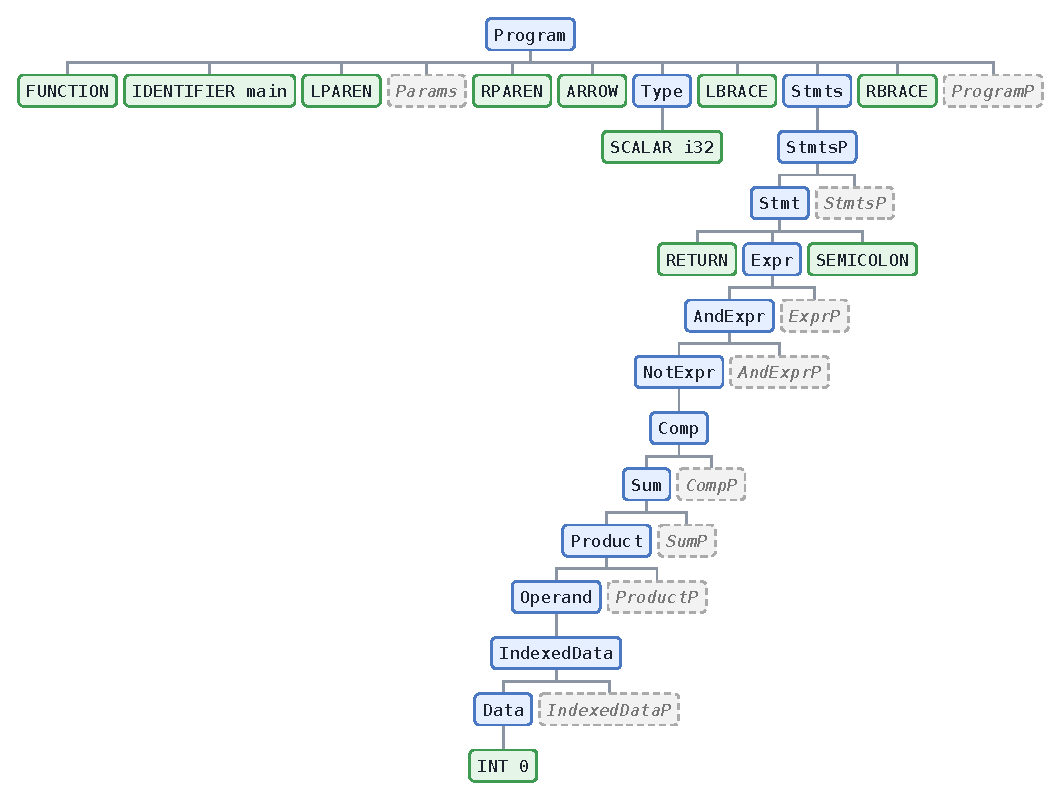
\includegraphics[width=0.8\linewidth]{resources/parse-tree-return0.pdf}
\caption{The parse tree of the minimal program.}
\label{fig:tree-tiny}
\end{figure}

\subsection{Operator Precedence}

The next example shows the precedence chain actually branching, rather
than passing straight through:

\begin{lstlisting}[caption={A declaration whose initializer branches.},
    label=lst:precedence-example]
function foo() -> i32 {
    i32 x = 1 + 2 * 3;
}
\end{lstlisting}

Figure~\ref{fig:tree-expr} draws its tree. The addition is the outer
operation: \nt{Sum} holds the \code{1}, and its \nt{SumP} child holds the
\code{+} together with the \nt{Product} for \code{2 * 3}, which is where
the multiplication is parsed, one level further down, before the addition
around it is complete. This is precedence shown structurally, with no
parentheses needed to force the multiplication to bind tighter.

\begin{figure}[H]
\centering
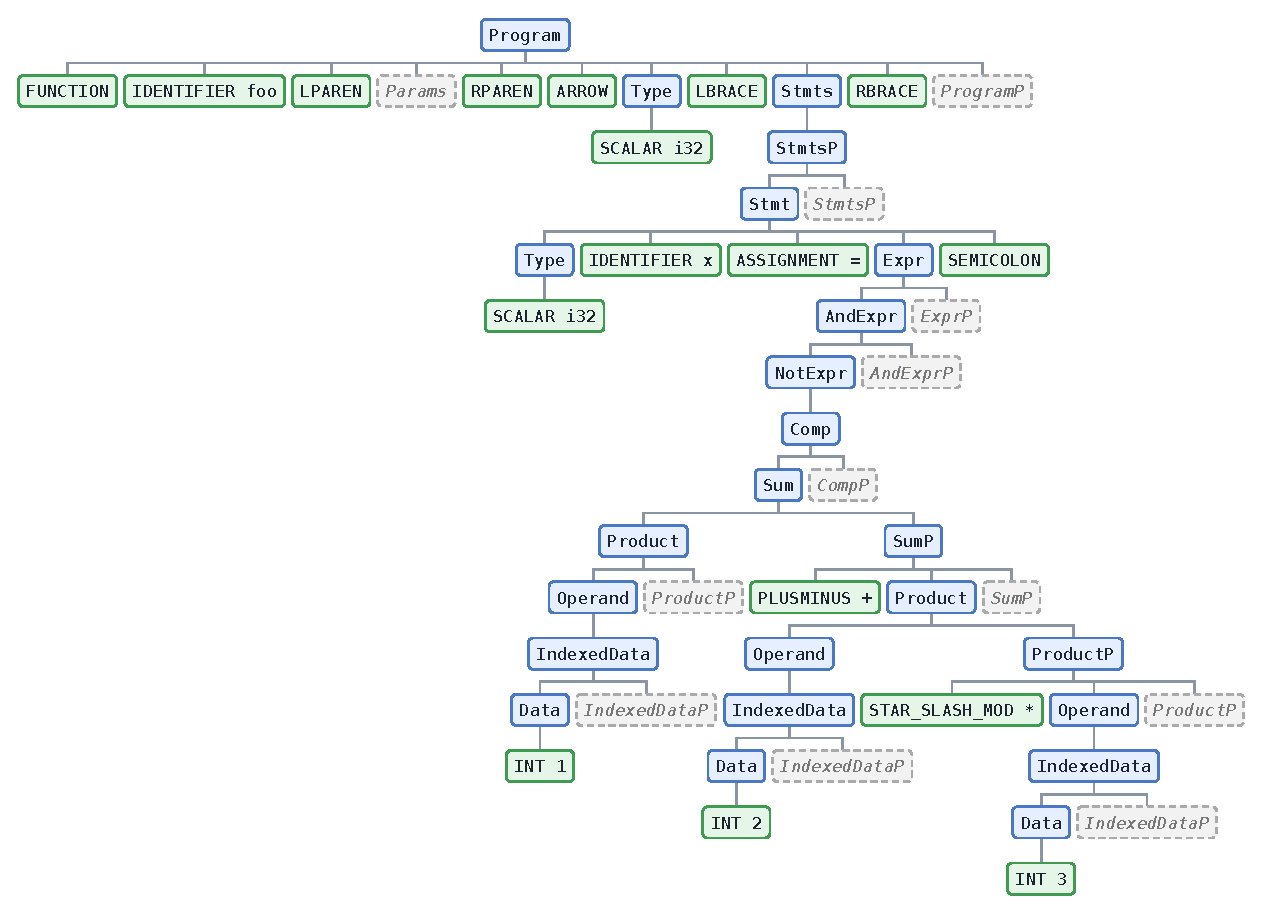
\includegraphics[width=\linewidth]{resources/parse-tree-expr.pdf}
\caption{The parse tree of Listing~\ref{lst:precedence-example}.}
\label{fig:tree-expr}
\end{figure}

In both figures, a nonterminal node is blue, a token is green, and a
nonterminal that derived the empty string is grey and dashed. Most of the
grey around the edges of Figures~\ref{fig:tree-tiny} and~\ref{fig:tree-expr}
is exactly this: nearly every \nt{...P} nonterminal in a short program
derives the empty string, since the recursion it stands for never runs for
more than a round or two.

\section{Parsers in the Real World}

The parser of OctaC, like its lexer, is hand-written rather than generated,
and deliberately small. This section looks at how parsers are built in
practice, and which simplifications ours makes.

\subsection{Parser Generators and Parsing Methods}

Many parsers are produced by a generator, the same way many lexers are.
Bison, upward compatible with the older Yacc, converts a grammar annotated
with actions into a parser, using LALR(1) tables by default
\cite{bison-manual}. LALR is a bottom-up method that accepts a larger class
of grammars than LL(1), at the cost of a less direct relationship between
the grammar and the code that results \cite{aho2006compilers}.

OctaC's grammar is restricted to LL(1) on purpose, so that the parser can
be a direct, hand-written translation of it, with no generated code and no
table beyond the one a human reads from the grammar itself.

\subsection{Hand-Written Recursive Descent}

Recursive descent is also a common choice for production compilers, not
only a teaching technique. Clang's parser is hand-written recursive
descent over the grammar of C and C++ \cite{clang-internals}, and CPython's
parser has been a hand-written PEG parser, a close relative of recursive
descent with unlimited lookahead and backtracking, since Python 3.9
\cite{python-pep617}. A hand-written parser gives the same advantages a
hand-written lexer does: direct control over error messages and recovery,
and no dependency on a generator as part of the build.

\subsection{Error Recovery}

Real parsers recover from a syntax error so that one run can report more
than the first one found, the same reason ours does. The general strategy,
skipping input until a token is reached that the grammar allows at some
enclosing point, is called panic mode recovery \cite{aho2006compilers}.
OctaC's parser is a direct application of it, with exactly two recovery
points chosen for the shape of the grammar: the end of a statement, and
the start of a function.

\subsection{Simplifications in OctaC}

Table~\ref{tab:parser-simplifications} summarizes the differences.

\begin{table}[H]
\centering
\small
\renewcommand{\arraystretch}{1.15}
\begin{tabular}{@{}>{\raggedright\arraybackslash}p{70pt}>{\raggedright\arraybackslash}p{190pt}>{\raggedright\arraybackslash}p{172pt}@{}}
\toprule
\textbf{Concern} & \textbf{Real-world parsers} & \textbf{OctaC} \\
\midrule
Construction & Generated from a grammar, or hand-written \cite{bison-manual,clang-internals} & Hand-written recursive descent \\
Grammar class & LALR or PEG, each more permissive than LL(1) \cite{aho2006compilers,python-pep617} & LL(1), by construction \\
Lookahead & Unbounded, with backtracking in a PEG parser \cite{python-pep617} & Exactly one token, never backtracks \\
Error recovery & Panic mode, or finer-grained strategies tuned per construct \cite{aho2006compilers} & Panic mode, at two recovery points \\
Tree & Often folded into an AST during parsing & A literal parse tree, one node per grammar symbol \\
Ambiguity & Resolved by precedence declarations in the generator & Resolved in the grammar itself, by construction \\
\bottomrule
\end{tabular}
\caption{Real-world parsers compared with the OctaC parser.}
\label{tab:parser-simplifications}
\end{table}


% Future chapters are added here as the language and compiler develop.
% \input{chp04-semantic-analysis}
% \input{chp05-code-generation}

\input{conclusion}
\addcontentsline{toc}{chapter}{Conclusion}

{
% The following prevents latex from splitting a bibliography entry with a page
% break
\interlinepenalty=10000
% Since we're using natbib in numbers mode, we don't need plainnat,
% which exists to feed authors and years back in to natbib.  As a
% result, it complains about entries without years, which we don't
% care about.
%\bibliographystyle{plainnat}
\bibliographystyle{plain}
\nocite{*}
\bibliography{bibliography}
\addcontentsline{toc}{chapter}{Bibliography}
}

\end{document}